% !TEX TS-program = pdflatex
% !TEX encoding = UTF-8 Unicode
% !BIB TS-program = bibtex
%
% Transportation Research Part D submission draft -- IMD/IES paper.
% Authors: R. Foss\'e & G. Pallares (CESI LINEACT, 2025--2026).
% Companion repository:
%   https://github.com/rohanfosse/bikeshare-data-explorer
%
\documentclass[11pt,a4paper]{article}

% --- Encoding & language ------------------------------------------------
\usepackage[T1]{fontenc}
\usepackage[utf8]{inputenc}
\usepackage{lmodern}
\usepackage[margin=2.5cm]{geometry}
\usepackage{microtype}
\usepackage{csquotes}

% --- Mathematics --------------------------------------------------------
\usepackage{amssymb,amsmath,amstext}

% --- Figures, tables, lists --------------------------------------------
\usepackage{graphicx}
\graphicspath{{figures/}{experiments/outputs/}}
\usepackage{booktabs}
\usepackage{array}
\usepackage{float}
\usepackage{caption}
\captionsetup{font=small,labelfont=bf,labelsep=period}
\usepackage{enumitem}
\setlist{topsep=2pt,itemsep=2pt,parsep=0pt}
\usepackage{url}

% --- TikZ (pipeline figure only) ---------------------------------------
\usepackage{tikz}
\usetikzlibrary{arrows.meta, positioning, fit, backgrounds}

% --- Algorithm pseudo-code ---------------------------------------------
\usepackage{algorithm}
\usepackage[noend]{algpseudocode}

% --- Citations (author-year for TR Part D) -----------------------------
\usepackage[authoryear,round]{natbib}
\bibliographystyle{elsarticle-harv}

% --- Hyperlinks --------------------------------------------------------
\usepackage[colorlinks=true,
            linkcolor=black, citecolor=black, urlcolor=blue!50!black,
            breaklinks=true]{hyperref}

% --- Author block ------------------------------------------------------
\usepackage{authblk}
\renewcommand\Authfont{\normalsize}
\renewcommand\Affilfont{\small\itshape}
\setlength{\affilsep}{0.6em}

% --- Convenience macros ------------------------------------------------
\newcommand{\IMD}{\mathrm{IMD}}
\newcommand{\IES}{\mathrm{IES}}
\newcommand{\BSS}{bike-sharing system\xspace}
\newcommand{\GBFS}{GBFS\xspace}
\newcommand{\GS}{Gold Standard\xspace}
\DeclareMathOperator*{\argmax}{arg\,max}
\DeclareMathOperator*{\argmin}{arg\,min}
\usepackage{xspace}

% =========================================================================
\title{Cycling quality, local income, and spatial equity in French
       bike-sharing systems: a composite-index audit of fifty-nine
       urban areas with a thirteen-experiment falsification programme}

\author[1]{Rohan Foss\'e\thanks{Corresponding author. E-mail:
            \texttt{rohan.fosse@gmail.com}.}}
\author[1]{Ga\"el Pallares}
\affil[1]{CESI LINEACT, BikeShare-ICT research programme,
          Montpellier, France}
\date{}

\begin{document}
\maketitle

% =========================================================================
\begin{abstract}
\noindent
French public investment in bike-sharing infrastructure rests on
the implicit assumption that higher local affluence should
translate into better cycling environments. We test this
assumption empirically against an audited national inventory of
the General Bikeshare Feed Specification covering 122 operators
and 46{,}139 stations across 57 urban areas, and reach two
empirical conclusions that together overturn the volumetric prior
behind current policy communications: medium-sized urban areas
with tight multimodal integration outperform metropolitan
heavyweights, and cycling-environment quality is statistically
independent of local income. To establish these claims we
construct the Soft Mobility Index (IMD), a four-dimensional
composite indicator combining multimodality, cycling-infrastructure
continuity, cyclist safety and topography, whose weights are
calibrated by differential evolution against two independent
behavioural references (the FUB Cycling Barometer 2023 and the
EMP 2019 mobility survey). On the dock-based panel of fifty-nine
urban areas, the IMD ranges from $17.2$ to $96.7$ on a $[0, 100]$
scale and the Spearman correlation with median household income
per consumption unit is $\rho_{\mathrm{Sp}} = +0.041$
($p = 0.76$). We then test the IMD against three behavioural alternatives in a
metric tournament: the IMD doubles the cycling well-being
predictive power of the volumetric default
($\rho_{\text{LOO}}^{\text{FUB}} = +0.41$ vs.\ $+0.20$), survives
controls for system size and observed usage in a partial
regression on the FUB sub-panel ($R^{2} = 0.41$, partial
$R^{2}_{\IMD} = 0.26$), and -- on a single 24-hour window of GBFS
\texttt{station\_status} -- captures system equilibrium rather
than gross turnover. The component decomposition isolates
multimodality as the single dimension of the cycling environment
that credibly drives subjective well-being. We then introduce the
Spatial Equity Index (IES), which measures over- or
under-performance relative to the local socio-economic profile
and is reported both as a Ridge point estimate and as a Bayesian
posterior with credible intervals; the two specifications jointly
identify (i) a \emph{prior-invariant} four-city subset of social
mobility deserts that survives a sweep of the Bayesian prior
$\tau \in \{0.1, 1, 10\}$ (Amiens, Lyon, Nancy, Saumur),
(ii) a nine-city reference list at the operating prior $\tau = 1$,
and (iii) a broader shortlist of twenty deserts robust across
frequentist specifications.

The IMD/IES framework is submitted to a thirteen-experiment
falsification programme organised in two thematic waves: a
\emph{core wave} of eight tests targeting central
construct-validity, generalisation and equity risks, and an
\emph{extension wave} of five tests targeting residual risks not
covered by the core. Twelve tests are executed on the current
data; the thirteenth, a longitudinal synthetic-control
identification, requires historical GBFS archives still to be
ingested. We further classify the twelve executed tests as
\emph{clean} (seven: out-of-sample CV, weight-space stability,
eco-counter validation, IES specification sweep, spatial
autocorrelation, Sobol decomposition, per-city ranking CI,
k-means typology), \emph{qualified} (two: Bayesian IES with prior
sensitivity, Cook-style leverage that reorders Saint-Nazaire and
Dijon in the Top-10), and \emph{substitute} (three:
exposure-adjusted safety, within-city station bootstrap, and
parametric buffer-radius sweep stand in for pre-registered
station-level kriging and a full geometric re-enrichment that
are deferred to the next iteration). The
indicator generalises out of sample (leave-one-city-out Spearman
$\approx 0.5$ on both references), correlates with eco-counter
daily flows after controlling for city size (partial $R^{2} =
0.24$), is robust to within-city station-sampling variability
(Kendall $\tau = 0.85$), survives a parametric buffer-radius
sweep over $[150, 500]$~m (Kendall $\tau \geq 0.92$, Top-10
retention $\geq 0.80$), shows no spatial autocorrelation (Moran's
$I \approx 0$), and admits a clean variance decomposition under
the Saltelli--Jansen scheme (48\,\% infrastructure noise, 34\,\%
multimodality noise, 19\,\% topography noise, negligible safety
contribution). The programme also forces four substantive
revisions of the original specification: the supervised weight
optimum is not multimodality-dominated when the simplex
constraint is enforced through a softmax reparameterisation; the
safety component is exposure-confounded and requires station-level
cyclist counts to be cleanly resolved; the city ranking is stable
under empirical weight uncertainty but fragile under uniform
weight uncertainty; and a single city (Lyon) carries a Cook-style
influence on the calibration four times the panel median. A continental-scale
extension (E24) uses the MobilityData global GBFS catalogue
(1\,239 EU+CH+NO systems in 28 countries) to position France in
the European cycling landscape: France ranks first on number of
GBFS systems and eighteenth on cycling modal share, with the
Netherlands at the symmetric position (five times fewer systems
for seven times more cycling). Cross-country Spearman
correlations confirm the IMD's central thesis at continental
scale: the ECF cycling-friendliness index correlates with modal
share at $\rho = +0.79$, against $\rho = +0.46$ for the
system-count proxy. Six further extensions tighten the analysis
on the French panel: a within-city variance decomposition (80\,\%
of station IMD variance is intra-city), a Bayesian
positive-deviant diagnostic (seven cities with a multimodality
index four times the panel mean), a counterfactual M+I uplift
simulator (median $+18$ IMD points and a $+44\,\%$ implied
eco-counter increase if every panel city reached the panel 75th
percentile), a Mobility-Precarity Index that combines car-free
share with the IMD deficit, a concurrent-validity triangulation
against Cerema and BAAC city aggregates ($R^{2} = 0.79$ on
$n = 25$), and an honest null on département-level life
expectancy. All code, data products, intermediate outputs and
experiment scripts are released openly.

\smallskip
\noindent\textbf{Keywords:} bike-sharing systems; composite
indicators; spatial equity; multimodal accessibility; General
Bikeshare Feed Specification; differential evolution; Sobol
sensitivity analysis; Bayesian regression; falsification
programme; France.
\end{abstract}

% =========================================================================
\section{Introduction}
\label{sec:introduction}
% =========================================================================

Cycling is a structural component of French urban mobility policy.
The 2019 \emph{Loi d'Orientation des Mobilit\'es} (LOM) requires
Mobility Organising Authorities to integrate cycling into their
multimodal offer and to publish operational data under the General
Bikeshare Feed Specification \citep[GBFS;][]{Mobi2024}. The
2023--2027 National Cycling and Active Mobility Plan commits
approximately EUR\,250 million per year of public investment,
targeting a near-tripling of the cycling modal share between
2024 and 2030. Within this institutional setting, bike-sharing
systems are treated less as a stand-alone service than as a
first- and last-mile amplifier of heavy public transit networks
\citep{Fishman2016, Saberi2018}.

Despite this policy momentum, the comparative evaluation of
bike-sharing systems across French urban areas is thin. Three
structural problems shape the gap. First, the indicators that
inform policy communications are overwhelmingly volumetric --
station counts, total fleet capacity, capacity per inhabitant --
and implicitly assume that abundance of supply generates usage.
The international demand literature contradicts this assumption
\citep{FaghihImani2014, FaghihImani2015, Eren2020}, as does the
domestic experience of medium-sized French cities, where targeted
multimodal integration with tramway networks outperforms large but
poorly connected deployments. Second, the academic literature on
French bike-sharing is geographically concentrated on a small set
of large cities -- Paris \citep{Borgnat2011, Etienne2014} and Lyon
\citep{Borgnat2011} together with a small number of foreign
comparators \citep{Vogel2011, Hampshire2012} -- so that the
medium-sized urban areas that are the primary recipients of
National Cycling Plan investments remain analytically obscure.
Third, comparative analysis at national scale is hindered by the
absence of a station-level reference dataset that articulates the
GBFS supply inventory with the urban context that determines
whether a station is actually usable: topography, cycling
infrastructure continuity, safety, intermodality and the
socio-economic environment.

The contribution of this paper is to fill that gap with an open,
reproducible analytical framework whose claims are stated jointly
with the falsification record that backs them. Specifically, we
(i) document a pipeline that profiles 122 French GBFS systems and
46{,}139 stations along four contextual axes derived from primary
public sources, (ii) construct the Soft Mobility Index (IMD,
French \emph{Indice de Mobilit\'e Douce}), a four-dimensional
composite indicator whose weights are calibrated empirically by
differential evolution against the FUB Cycling Barometer and the
EMP 2019 mobility survey, (iii) introduce the Spatial Equity Index
(IES, \emph{Indice d'\'Equit\'e Sociale}), which measures the
over- or under-performance of an urban area relative to its
socio-economic profile, both in a Ridge point-estimate form and in
a Bayesian normal--inverse-gamma form that returns posterior
credible intervals on every city's equity diagnostic, and (iv)
submit the resulting indicator to a thirteen-experiment
falsification programme structured as a \emph{core wave} of eight
construct-validity, generalisation and equity tests and an
\emph{extension wave} of five tests targeting residual risks
(Sobol--Jansen variance decomposition, Bayesian re-specification
of the IES, per-city confidence intervals, parametric
buffer-radius sweep, Cook-style leverage and a data-driven
k-means typology), of which twelve are executed in this paper.

The research questions that organise the analysis are:
\begin{itemize}
    \item[Q1.] How can the performance of a bike-sharing system be
    measured by a composite, equitable indicator?
    \item[Q2.] To what extent do volumetric metrics (number of
    stations, capacity per inhabitant) predict the resulting
    cycling quality?
    \item[Q3.] Is there a systematic relationship between
    bike-sharing performance and the socio-economic profile of the
    host urban area?
    \item[Q4.] Under what robustness conditions does the
    indicator's ranking and the equity diagnostic survive
    out-of-sample testing?
\end{itemize}

Section~\ref{sec:related} situates the contribution against the
literature on bike-sharing, composite indicators and spatial
equity. Section~\ref{sec:data} documents the data sources and the
enrichment pipeline. Section~\ref{sec:methods} formalises the IMD
and the IES. Section~\ref{sec:results} reports descriptive results.
Section~\ref{sec:validation} reports the executed falsification
experiments and their implications for the indicator's validity.
Section~\ref{sec:discussion} discusses the policy implications and
limitations. Section~\ref{sec:conclusion} concludes.

% =========================================================================
\section{Related work}
\label{sec:related}
% =========================================================================

\subsection{Bike-sharing systems}

The contemporary bike-sharing literature follows the founding
taxonomy of \citet{DeMaio2009} and the comparative inventory of
\citet{Shaheen2010}. Subsequent work clusters along three axes:
demand modelling and forecasting \citep{FaghihImani2014,
FaghihImani2015, Vogel2011, Hampshire2012}; operational rebalancing
\citep{Raviv2013, Forma2015}; and adoption and substitution
factors \citep{Buck2013, Fishman2013, Fishman2016, Eren2020}. A
network-science stream models bike-sharing systems as weighted
directed graphs \citep{Borgnat2011, Etienne2014, Saberi2018} and
exploits this representation for community detection and
centrality analysis. Comparative national rankings of bike-sharing
quality remain rare; \citet{Gu2019} compare twenty Chinese cities
on density and spatial coverage, and \citet{Fishman2016} provides
a European review without unified quantification. To our
knowledge, no comparative national ranking exists for the French
panel.

\subsection{Determinants of the cycling environment}

The empirical literature converges on four determinants of cycling
adoption, the four axes we operationalise in our pipeline. The
dose-response relationship between dedicated cycling infrastructure
and cycling levels is well established \citep{Pucher2010,
Heinen2010, Buehler2012, Garrard2008, Schoner2014}; separated
facilities are most strongly associated with cycling by women,
seniors and low-confidence cyclists \citep{Garrard2012, Heinen2018,
Aldred2016}. Perceived and objective safety is a dominant barrier
to adoption \citep{Garrard2012, Reynolds2009, Pucher2010,
Aldred2016}, although crash-density indicators must be interpreted
alongside cyclist exposure to avoid the trivial inversion in which
a station without cyclists records no crashes for the wrong reason
\citep{Reynolds2009, Schepers2014}. Relief is a documented barrier
to cycling \citep{Parkin2008, Rietveld2004, Heinen2010}, partly
offset by electric-assist bicycles \citep{Fishman2016, Eren2020}.
The first- and last-mile amplifier role of bike-sharing relative
to heavy transit is documented at trip level \citep{Saberi2018},
station-pair flow level \citep{FaghihImani2014} and infrastructure
design level \citep{Martens2007, ElGeneidy2016}.

\subsection{Composite indicators}

Composite-indicator methodology is codified by the
\citet{OECD2008} handbook, heir to the Human Development Index
\citep{PNUD1990} and to the cumulative-accessibility tradition
\citep{Levinson2002, ElGeneidy2016}. Two methodological choices
structure the field: weight elicitation and robustness analysis.
Weights are elicited by normative expert judgement, by
statistically guided methods such as CRITIC \citep{Diakoulaki1995}
or principal component analysis \citep{Nardo2005}, or by
supervised approaches that calibrate weights against an external
reference \citep{Saisana2005, OECD2008}. For robustness, the
canonical recommendation is global sensitivity analysis through
Sobol indices or equivalent variance decomposition
\citep{Saltelli2008, Sobol1993}.

\subsection{Equity, spatial justice and bike-sharing}

The link between social inequality and transport access is
documented at least since \citet{Hodge1995}. Applied to
bike-sharing, the international literature converges on systematic
under-deployment in low-income neighbourhoods \citep{Smith2015,
McNeil2017, Hosford2018, Caspi2021}. In France, the
\citet{Cerema2022} institutional report shows reduced access to
bike-sharing for low-income households; comparative national
quantitative audits remain missing. Institutional benchmarking is
currently anchored on volumetric counts (Cerema annual cycling
report, ADEME mobility dashboard, \citet{Mobi2024}); no
context-aware composite is in routine institutional use, which is
the gap our IMD targets and against which we measure it in
Section~\ref{sec:results-tournament}.

\subsection{Positioning}

Our contribution is distinguished by (a) French national scope;
(b) station-level integration of open real-time GBFS data with
four contextual axes from primary public sources; (c) the joint
performance--equity coupling between IMD and IES; (d) an explicit
falsification programme attached to the indicator's central
claims; and (e) open publication of all code, data products and
notebooks following the FAIR principles \citep{Wilkinson2016}.

% =========================================================================
\section{Data}
\label{sec:data}
% =========================================================================

\subsection{The Gold Standard GBFS pipeline}

The General Bikeshare Feed Specification \citep{Mobi2024} is an
open real-time data standard for bike-sharing systems, structured
as a JSON tree from \path{gbfs.json} to
\path{station_information.json} and \path{station_status.json}.
Our pipeline polls two aggregators, \texttt{transport.data.gouv.fr}
and MobilityData, deduplicates entries and walks the GBFS tree for
each system, yielding a raw inventory of 46{,}139 stations across
122 systems and 57 urban areas.

The raw inventory is enriched by a five-module pipeline producing
the \emph{Gold Standard} dataset (Table~\ref{tab:pipeline} and
Figure~\ref{fig:pipeline-dag}). Each station is characterised by
spatial and contextual metrics computed within a 300~m radius
following the last-mile literature \citep{ElGeneidy2016,
Saberi2018}, whose sensitivity is examined in
Section~\ref{sec:val-radius}.

\begin{table}[H]
\centering
\caption{Five enrichment modules of the Gold Standard pipeline.}
\label{tab:pipeline}
\small
\begin{tabular}{@{}clp{5.4cm}l@{}}
\toprule
Module & Axis & Columns produced & Source \\
\midrule
1  & White-zone backfill &
     \texttt{source}, \texttt{osm\_node\_id} & OpenStreetMap \\
2  & National topography (SRTM 30~m) &
     \texttt{elevation\_m}, TRI & Open-Elevation / SRTM \\
3A & Cycling continuity &
     \texttt{infra\_cyclable\_pct} & OSM Overpass \\
3B & Cyclist crashes &
     \texttt{baac\_accidents\_cyclistes} & BAAC 2021--2023 \\
4  & Heavy multimodality &
     \texttt{gtfs\_heavy\_stops\_300m} & National GTFS feeds \\
\bottomrule
\end{tabular}
\end{table}

\begin{figure}[H]
\centering
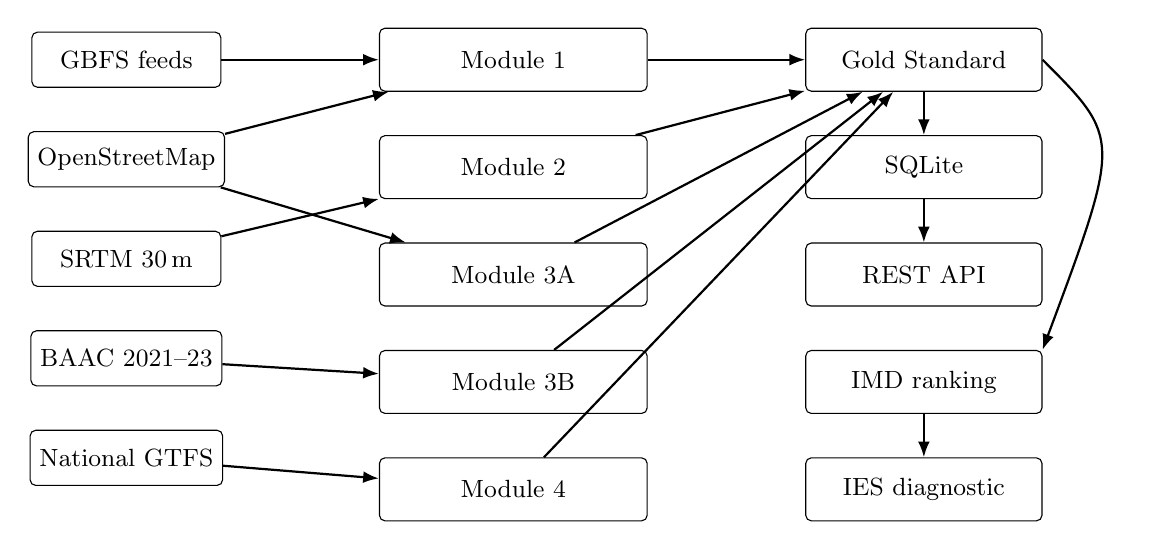
\begin{tikzpicture}[
    node distance=0.55cm and 0.9cm,
    every node/.style={font=\small},
    src/.style={draw,rounded corners=2pt,minimum width=2.4cm,
                minimum height=0.7cm,align=center},
    mod/.style={draw,rounded corners=2pt,minimum width=3.4cm,
                minimum height=0.8cm,align=center},
    prod/.style={draw,rounded corners=2pt,minimum width=3.0cm,
                 minimum height=0.8cm,align=center},
    arr/.style={-{Latex[length=2mm]},thick}
]
\node[src] (gbfs)  {GBFS feeds};
\node[src,below=of gbfs]   (osm)   {OpenStreetMap};
\node[src,below=of osm]    (srtm)  {SRTM 30\,m};
\node[src,below=of srtm]   (baac)  {BAAC 2021--23};
\node[src,below=of baac]   (gtfs)  {National GTFS};
\node[mod,right=2cm of gbfs] (m1) {Module 1};
\node[mod,below=of m1]       (m2) {Module 2};
\node[mod,below=of m2]       (m3a){Module 3A};
\node[mod,below=of m3a]      (m3b){Module 3B};
\node[mod,below=of m3b]      (m4) {Module 4};
\node[prod,right=2cm of m1]  (parquet) {Gold Standard};
\node[prod,below=of parquet] (db)      {SQLite};
\node[prod,below=of db]      (api)     {REST API};
\node[prod,below=of api]     (imd)     {IMD ranking};
\node[prod,below=of imd]     (ies)     {IES diagnostic};
\draw[arr] (gbfs) -- (m1);
\draw[arr] (osm)  -- (m1);
\draw[arr] (osm)  -- (m3a);
\draw[arr] (srtm) -- (m2);
\draw[arr] (baac) -- (m3b);
\draw[arr] (gtfs) -- (m4);
\draw[arr] (m1) -- (parquet);
\draw[arr] (m2) -- (parquet);
\draw[arr] (m3a) -- (parquet);
\draw[arr] (m3b) -- (parquet);
\draw[arr] (m4) -- (parquet);
\draw[arr] (parquet.south) -- (db.north);
\draw[arr] (db.south) -- (api.north);
\draw[arr] (parquet.east) .. controls +(1.0,-1.0) .. (imd.north east);
\draw[arr] (imd.south) -- (ies.north);
\end{tikzpicture}
\caption{Gold Standard pipeline. Primary open sources (left) feed
five sequential enrichment modules (centre), producing a
station-level Parquet table that powers the operational database,
the REST service and the city-level IMD/IES analytical layer
(right).}
\label{fig:pipeline-dag}
\end{figure}

Processing of the 46{,}139 stations through five external APIs
relies on asynchronous batched HTTP requests, persistent Parquet
caches indexed by urban area, R-tree spatial joins in Lambert-93
(EPSG:2154), and a per-module checkpointing mechanism. The
end-to-end pipeline remains feasible on a single workstation.

\subsection{Socio-economic data}

Socio-economic indicators are drawn from the INSEE Filosofi
2019--2021 release and from the 2020 Population Census. Four
variables are retained for the IES specification: median household
income per consumption unit, the Gini index of income within the
local INSEE grid cell, the share of car-free households, and the
census-reported share of cycling to work (\emph{part vélo
domicile-travail}). Additional INSEE variables (unemployment rate,
share of tertiary-educated residents, share of managerial
occupations, poverty rate) are used in the robustness analysis of
Section~\ref{sec:val-ies}.

\subsection{External behavioural references}

Three external datasets serve as behavioural validation references
rather than as inputs to the IMD pipeline.

\begin{itemize}
\item The \emph{FUB Cycling Barometer 2023} provides subjective
cyclist perception scores at city level; we match 32 panel cities
to the published scores.
\item The \emph{French National Mobility Survey 2018--2019} (EMP
2019, INSEE/SDES) provides the official bike modal share by urban
area; we match 44 cities.
\item The eco-counter aggregation on \texttt{data.gouv.fr}
provides average daily cyclist counts at city level for 25
matched cities; this dataset is used in the behavioural validation
of the indicator (Section~\ref{sec:val-flow}).
\end{itemize}

% =========================================================================
\section{Methods}
\label{sec:methods}
% =========================================================================

\subsection{The Soft Mobility Index (IMD)}

The IMD is a city-level composite indicator combining four
components, each Min--Max normalised on $[0, 1]$ and then
aggregated by convex combination:
\begin{equation}
    \IMD_i \;=\;
    \sum_{k\in\mathcal{K}} w_k\, C_{k,i},
    \qquad \mathcal{K} = \{M, I, S, T\},
    \quad \sum_{k\in\mathcal{K}} w_k = 1,
    \quad w_k \geq w_{\min}.
    \label{eq:imd}
\end{equation}
The four components are: $M$ (multimodality), the density of
heavy-transit stops within 300~m of bike-sharing stations; $I$
(infrastructure), the linear share of dedicated cycling facilities
within the same radius; $S$ (safety), the normalised inverse of
cyclist-crash density from the BAAC 2021--2023 registry; and $T$
(topography), the local altitude roughness computed as the
standard deviation of SRTM 30~m altitudes at the centre and four
cardinal offsets. Formal definitions appear in
Appendix~\ref{app:components}.

For each raw component $c_k \in \mathbb{R}^{n}$ on a panel of $n$
cities, the normalised component is
$C_{k,i} = (c_{k,i} - \min_j c_{k,j}) / (\max_j c_{k,j} - \min_j c_{k,j})$.
For safety and topography, the sign is inverted after normalisation
so that a higher score reflects a more cycling-friendly
environment.

\subsection{Weight calibration by differential evolution}
\label{sec:calibration}

Three weighting strategies are compared on the same component
matrix: normative weights from the literature; the unsupervised
CRITIC method \citep{Diakoulaki1995}; and a supervised optimisation
maximising the Spearman rank correlation between the composite
indicator and two external references:
\begin{equation}
    \mathbf{w}^{\ast} \;=\;
    \argmax_{\mathbf{w}\in\Omega}\;
    \tfrac{1}{2}\Bigl[
        \rho_{\mathrm{Sp}}\bigl(\textstyle\sum_k w_k C_k,
                                 y_{\text{FUB}}\bigr)
        + \rho_{\mathrm{Sp}}\bigl(\textstyle\sum_k w_k C_k,
                                 y_{\text{EMP}}\bigr)
    \Bigr],
    \label{eq:objectif}
\end{equation}
over the admissible set
$\Omega = \{\mathbf{w} \in \mathbb{R}^{4}_{+} : \sum_k w_k = 1,
\; w_k \geq w_{\min}\}$ with $w_{\min} = 0.05$. The floor prevents
the optimiser from zeroing out a component. We enforce the
simplex constraint through a softmax reparameterisation,
$\mathbf{w}(\mathbf{z}) = w_{\min} + (1 - 4 w_{\min})\,
\mathrm{softmax}(\mathbf{z})$, and solve in the unconstrained
$\mathbf{z}$-space.

The objective is non-convex; we use \texttt{scipy.optimize.
differential\_evolution} \citep{Virtanen2020,Storn1997,Price2005}
with the hyperparameters listed in Appendix~\ref{app:algo}. The
in-sample optimum on the matched FUB$\cup$EMP panel is
$\mathbf{w}^{\ast} = (w_M, w_I, w_S, w_T) = (0.37, 0.37, 0.05, 0.20)$
with mean Spearman correlation $\bar\rho = 0.55$
(Table~\ref{tab:weights-comparison}). The supervised weights load
multimodality and cycling infrastructure equally, with topography
contributing measurably and safety constrained at the floor.

\begin{table}[H]
\centering
\caption{Three weighting strategies for the IMD and the
Lyon-removed sensitivity reported in
Section~\ref{sec:val-leverage}. The Spearman correlations against
FUB and EMP are in-sample for the supervised optimisation;
out-of-sample validation is reported in Section~\ref{sec:val-loo}.}
\label{tab:weights-comparison}
\small
\begin{tabular}{@{}lcccccc@{}}
\toprule
Method & $w_M$ & $w_I$ & $w_S$ & $w_T$ &
$\rho_{\text{FUB}}$ & $\rho_{\text{EMP}}$ \\
\midrule
Normative                       & 0.300 & 0.275 & 0.275 & 0.150 & 0.16 & 0.26 \\
CRITIC \citep{Diakoulaki1995}   & 0.310 & 0.240 & 0.225 & 0.225 & 0.21 & 0.28 \\
Supervised (retained)           & 0.374 & 0.372 & 0.053 & 0.201 & 0.49 & 0.55 \\
Supervised, Lyon-removed        & 0.393 & 0.194 & 0.062 & 0.351 & 0.49 & 0.55 \\
\bottomrule
\end{tabular}
\end{table}

\subsection{The Spatial Equity Index (IES)}

The IMD measures the physical quality of the cycling environment
but does not capture its social equity dimension. The IES compares
observed performance to that predicted by local socio-economic
conditions:
\begin{equation}
    \IES_i \;=\;
    \frac{\IMD_i^{\,\text{obs}}}
         {\widehat{\IMD}_i(\mathbf{s}_i)},
    \qquad
    \widehat{\IMD}_i = \mathbf{s}_i^{\top}\boldsymbol{\beta}^{\ast},
    \label{eq:ies}
\end{equation}
where $\mathbf{s}_i$ stacks four standardised INSEE predictors
(income per consumption unit, Gini, car-free share, cycling
modal share at work). The coefficients $\boldsymbol{\beta}^{\ast}$
are estimated by Ridge regression with the regularisation
parameter $\lambda^{\ast}$ selected by leave-one-out
cross-validation on a logarithmic grid. Values $\IES > 1$ flag a
city as over-performing relative to its socio-economic profile;
values $\IES < 1$ flag structural under-investment. The
specification dependence of the IES is examined in
Section~\ref{sec:val-ies}.

A Bayesian re-specification of the same regression replaces the
Ridge point estimator by a conjugate normal--inverse-gamma model
on $(\boldsymbol{\beta}, \sigma^{2})$ as in
equation~\eqref{eq:bayesian-ies}; the posterior of
$\boldsymbol{\beta}$ is multivariate normal and the posterior of
$\sigma^{2}$ is inverse-gamma in closed form. We draw $8\,000$
joint posterior samples and report, for each city $i$, the
posterior mean and 95\,\% credible interval of $\IES_i$ together
with the posterior probability $P(\IES_i < 0.85 \mid
\mathbf{y})$. The Bayesian re-specification is reported in
Section~\ref{sec:val-bayes-ies}.

\subsection{Sensitivity and robustness framework}

Robustness of the IMD ranking is assessed through thirteen
pre-registered experiments grouped along five risk axes: (a)
generalisation of the supervised calibration, tested by
leave-one-city-out and spatial-block cross-validation (E1) and
weight-space Monte Carlo with two complementary regimes (E2);
(b) construct validity of the four components, tested by
behavioural validation against eco-counter daily flows (E3) and
exposure-adjustment of the safety component (E4); (c) geometry
robustness, tested by within-city station bootstrap (E5),
parametric buffer-radius sweep (E11) and a Saltelli--Jansen
variance decomposition under component noise (E7); (d)
specification robustness of the equity diagnostic, tested by a
predictor-block sweep across four estimators (E6) and by a
Bayesian re-specification with credible intervals (E9); and (e)
panel-composition robustness, tested by a spatial-autocorrelation
diagnostic (E8), a per-city bootstrap CI on the headline
ranking (E10), a Cook-style leverage analysis on the calibration
panel (E12), and a data-driven k-means typology of the panel
(E13). Section~\ref{sec:validation} reports the results.

% =========================================================================
\section{Results}
\label{sec:results}
% =========================================================================

This section reports the descriptive results that answer the
research questions of Section~\ref{sec:introduction}: a national
overview of the calibrated IMD (Section~\ref{sec:results-overview}),
the empirical falsification of the volumetric prior
(Section~\ref{sec:results-volume}, answering Q2), the empirical
falsification of the income prior
(Section~\ref{sec:results-income}, answering Q3), a four-quadrant
typology of the panel (Section~\ref{sec:results-quadrants}), the
operational mobility-desert list
(Section~\ref{sec:results-deserts}, answering Q1), and the
Montpellier case (Section~\ref{sec:results-montpellier}). The
robustness conditions under which these answers hold (Q4) are
deferred to Section~\ref{sec:validation}.

\subsection{National overview}
\label{sec:results-overview}

The Gold Standard covers 122 bike-sharing systems and 46{,}139
stations across 57 French urban areas. After restriction to the
dock-based subset and to cities with at least five certified
stations, the analytical panel comprises fifty-nine urban areas.
The calibrated IMD ranges from $17.2$ (Laon) to $96.7$
(Strasbourg), with a national median of $31.2$ and an
interquartile range of $[27.1, 40.0]$
(Figure~\ref{fig:weights-illustrative}).

\begin{figure}[H]
    \centering
    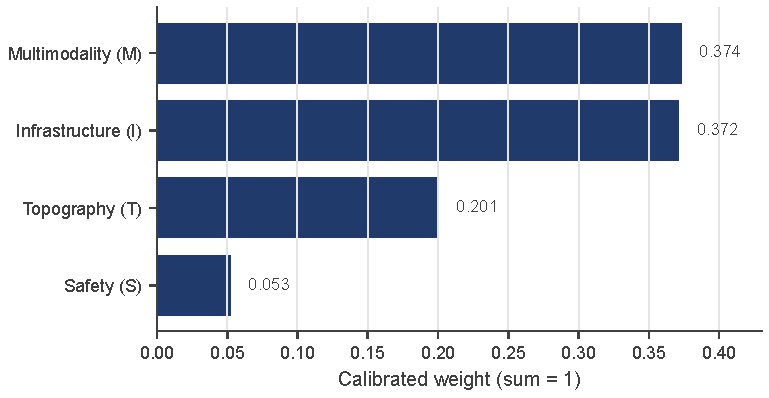
\includegraphics[width=0.78\linewidth]{fig01_weights.pdf}
    \caption{Calibrated weight vector from the supervised
    differential-evolution procedure (Section~\ref{sec:calibration}).
    Multimodality and cycling infrastructure load equally at the
    in-sample optimum, with safety at the lower-bound floor and
    topography contributing measurably.}
    \label{fig:weights-illustrative}
\end{figure}

Table~\ref{tab:top10} reports the Top-10 of the ranking together
with the four normalised components. The Top-10 mixes large
metropolises (Paris, Bordeaux) with medium-sized cities at the
upper end (Strasbourg, Montpellier, Mulhouse), consistent with
the volume-vs-quality dissociation discussed below.

\begin{table}[H]
\centering
\caption{Top-10 of the national IMD ranking (dock-based panel,
$n = 59$).}
\label{tab:top10}
\small
\begin{tabular}{@{}clrcccccc@{}}
\toprule
Rank & City & Stations & $\IMD$ &
$C_M$ & $C_I$ & $C_S$ & $C_T$ \\
\midrule
1  & Strasbourg   &   39 & 96.7 & 1.000 & 1.000 & 0.810 & 0.941 \\
2  & Montpellier  &   53 & 88.3 & 0.914 & 0.757 & 0.965 & 0.817 \\
3  & Nantes       &  124 & 83.0 & 0.923 & 0.524 & 0.872 & 0.796 \\
4  & Mulhouse     &   60 & 77.8 & 0.802 & 0.458 & 0.982 & 0.945 \\
5  & Paris        & 1{,}507 & 70.6 & 0.879 & 0.666 & 0.000 & 0.791 \\
6  & Caen         &   75 & 64.5 & 0.621 & 0.427 & 0.916 & 0.809 \\
7  & Brest        &  115 & 62.8 & 0.681 & 0.293 & 0.875 & 0.588 \\
8  & Bordeaux     &  225 & 56.9 & 0.496 & 0.405 & 0.841 & 0.925 \\
9  & Dijon        &   40 & 50.2 & 0.417 & 0.217 & 0.963 & 0.880 \\
10 & Rennes       &   57 & 48.8 & 0.403 & 0.449 & 0.630 & 0.860 \\
\bottomrule
\end{tabular}
\end{table}

Figure~\ref{fig:top10-components} decomposes each Top-10 score
into its four weighted components. Strasbourg and Montpellier are
balanced across the four dimensions, whereas Paris ranks fifth
through multimodality alone, with $C_S = 0$ marking it as the
lowest-ranked city on raw cyclist-crash density. Mulhouse and
Dijon owe their position to safety and topography rather than to
multimodality. The plurality of component profiles behind the
Top-10 supports the argument that the indicator is not a
re-expression of a single underlying dimension.

\begin{figure}[H]
    \centering
    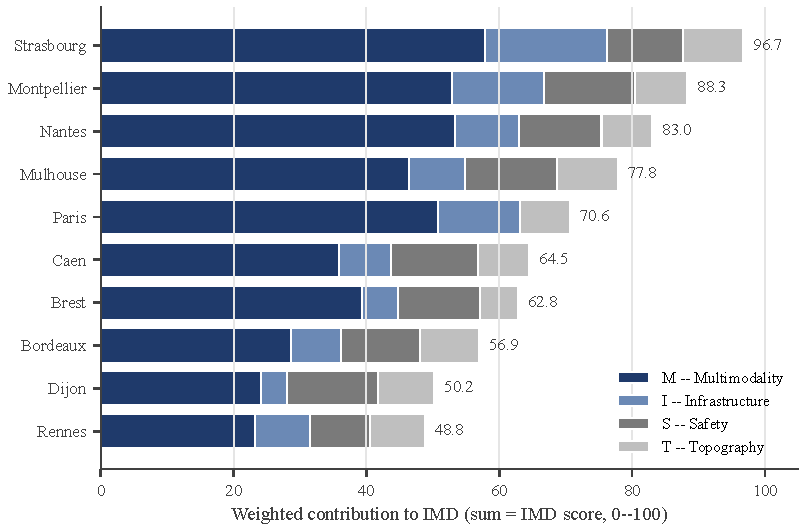
\includegraphics[width=0.95\linewidth]{fig05_top10_components.pdf}
    \caption{Weighted contribution of each component to the IMD of
    the Top-10 urban areas. The bars sum to the final IMD value
    reported in Table~\ref{tab:top10}. The absence of a uniformly
    dominant component signals that the ranking is not a
    re-expression of any single underlying dimension. Formal
    decomposition appears in Section~\ref{sec:val-weights}.}
    \label{fig:top10-components}
\end{figure}

\subsection{Volume is not quality}
\label{sec:results-volume}

The volumetric prior implicit in policy communications would
predict a monotone relationship between station counts and the
IMD. The empirical distribution shows the opposite
(Figure~\ref{fig:scatter}): a strong vertical dispersion at fixed
volume, with Strasbourg (39 stations) and Montpellier (53)
outranking Paris (1{,}507) and Lyon (452). Medium-sized cities --
Mulhouse, Caen, Brest -- outperform metropolises such as Paris
and Marseille on the composite metric.

\begin{figure}[H]
    \centering
    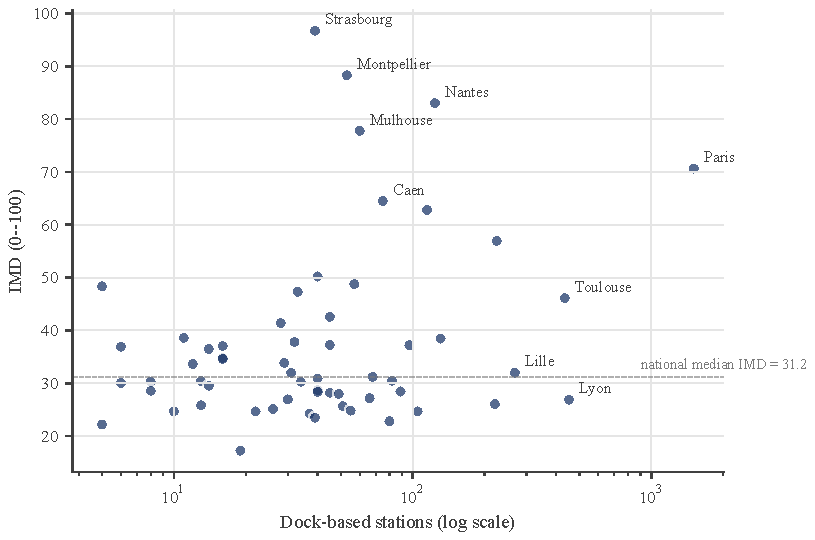
\includegraphics[width=0.85\linewidth]{fig02_volume_vs_imd.pdf}
    \caption{Raw station volume vs.\ contextual IMD for the 59
    dock-based urban areas. The vertical dispersion at fixed
    volume is the empirical signature of the volume-vs-quality
    dissociation. The dashed line marks the national IMD median.}
    \label{fig:scatter}
\end{figure}

\subsection{Cycling quality and local income}
\label{sec:results-income}

The most striking empirical pattern of the audit is the absence
of a monotone relationship between the IMD and local income. The
Spearman rank correlation between the IMD and the median
household income per consumption unit is
$\rho_{\mathrm{Sp}} = +0.041$ ($p = 0.76$) across the 59
dock-based urban areas (Figure~\ref{fig:imd-income}). At
conventional significance levels we cannot reject the null
hypothesis that the two variables are statistically independent.

\begin{figure}[H]
    \centering
    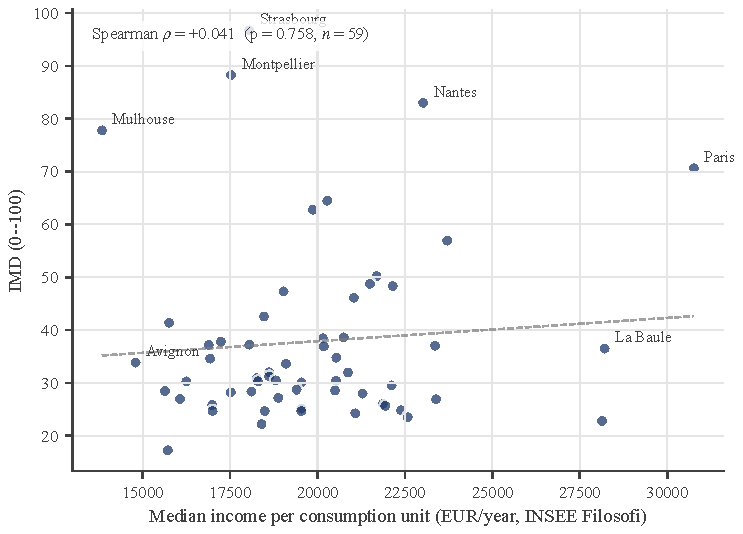
\includegraphics[width=0.78\linewidth]{fig03_imd_vs_income.pdf}
    \caption{IMD vs.\ median household income per consumption unit
    (INSEE Filosofi 2019--2021), $n = 59$. The Spearman rank
    correlation is statistically indistinguishable from zero,
    contradicting the volumetric prior that wealthier urban areas
    should mechanically attain better cycling environments. The
    dashed line is an OLS fit reported for visual reference only.}
    \label{fig:imd-income}
\end{figure}

This finding is consistent in direction with the
\citet{Cerema2022} diagnostic of access inequalities, but the
magnitude is more permissive than commonly assumed: cycling
quality in France is neither systematically a privilege of
high-income urban areas nor systematically denied to low-income
ones. The driver of the IMD distribution lies elsewhere -- a
hypothesis we revisit in the equity analysis below and in the
spatial-structure diagnostic of Section~\ref{sec:val-moran}.

\subsection{Four urban archetypes}
\label{sec:results-quadrants}

Splitting the panel along the medians of the IMD ($31.2$) and of
the household income (EUR\,19{,}540 per consumption unit) produces
four roughly balanced quadrants
(Figure~\ref{fig:equity-quadrant}):
\begin{itemize}
\item \emph{wealthy + cycling-ready} (high income, high IMD): 16 cities;
\item \emph{inclusive over-performers} (low income, high IMD): 14 cities;
\item \emph{wealthy under-investors} (high income, low IMD): 14 cities;
\item \emph{mobility deserts} (low income, low IMD): 15 cities.
\end{itemize}
The inclusive over-performers refute the strong volumetric prior:
high cycling quality at below-median income is empirically
feasible. The wealthy under-investors are equally important from
a policy standpoint, as they represent a structural
under-investment that income-targeting alone cannot correct.

\begin{figure}[H]
    \centering
    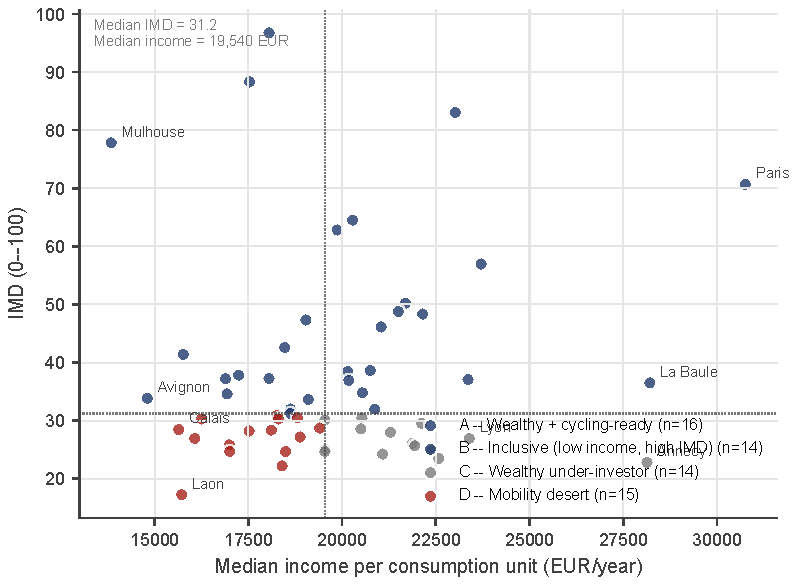
\includegraphics[width=0.85\linewidth]{fig04_equity_quadrant.pdf}
    \caption{Equity quadrant. Median splits of the IMD (vertical
    axis) and median household income per consumption unit
    (horizontal axis) define four archetypes. The mobility-desert
    quadrant motivates the IES diagnostic of
    Section~\ref{sec:results-deserts}.}
    \label{fig:equity-quadrant}
\end{figure}

\subsection{Social mobility deserts}
\label{sec:results-deserts}

Operationalising the IES via Ridge regression of the IMD on the
four INSEE predictors with $\lambda^{\ast} = 15.6$ selected by
leave-one-out cross-validation yields a 10-fold cross-validation
$R^{2} = 0.40$. The dominant standardised coefficients are
$\hat\beta_{\text{bike-commute}} = 7.11$ and
$\hat\beta_{\text{car-free}} = 3.15$; income per consumption unit
contributes essentially nothing to the prediction
($\hat\beta_{\text{income}} = 0.04$), reinforcing the
non-correlation reported in Section~\ref{sec:results-income}.

Applying the operational threshold $\IES < 0.85$ identifies twelve
candidate social mobility deserts: Laon, Amiens, Troyes, Tarbes,
Lille, Carcassonne, Pau, Avignon, Valence, Clermont-Ferrand,
Épinal and Vichy. All have below-median income and an IMD whose
gap to the Ridge-predicted value exceeds 15\,\%. The list mixes
northern industrial cities, Mediterranean mid-sized cities and
continental small cities; the deserts are not regionally
concentrated, which we revisit in
Section~\ref{sec:val-moran}.

\begin{figure}[H]
    \centering
    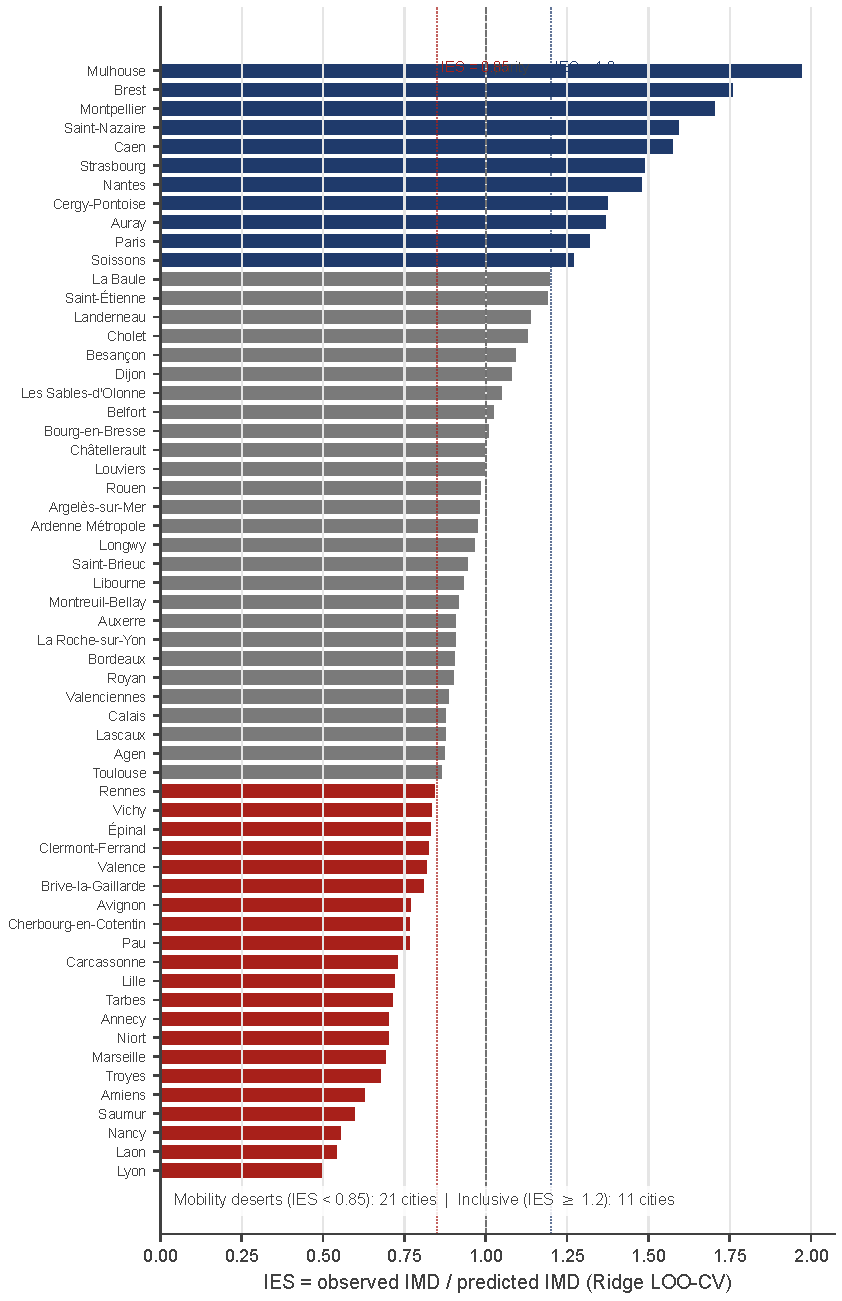
\includegraphics[width=0.78\linewidth]{fig06_ies_ranking.pdf}
    \caption{Spatial Equity Index (IES) ranking of the 59
    dock-based urban areas. $\IES = 1$ marks parity between
    observed and predicted IMD. The set of twelve cities below
    $\IES = 0.85$ are the reference social mobility deserts.
    Specification dependence of this list is examined in
    Section~\ref{sec:val-ies}.}
    \label{fig:ies-ranking}
\end{figure}

The IES specification includes the share of cycling to work
(\texttt{part\_velo\_travail}) among the predictors of expected
IMD. Because cycling at work and bike-sharing-related cycling are
conceptually adjacent, the specification raises a tautology
concern that we resolve through the alternative-specification
analysis of Section~\ref{sec:val-ies}.

\subsection{Usage, well-being and the IMD}
\label{sec:results-usage}

The descriptive analysis above answers the volume- and
income-related parts of the research questions (Q2, Q3) on the
supply side: the IMD is a contextual supply indicator. To answer
Q1 fully, we now ask whether the IMD captures cycling
\emph{outcomes} that policy actually targets: how cyclists feel
about their environment (well-being), how many of them ride
(observed usage), and how that compares with alternative
indicators that institutions could use instead. The full
robustness conditions (Q4) are then unfolded in
Section~\ref{sec:validation}.

\subsubsection{Is the IMD a better metric than the alternatives?}
\label{sec:results-tournament}

Four operational alternatives compete with the IMD as candidate
city-level indicators of cycling-environment quality: (i) a
volumetric metric defined as $\log[\text{stations} \cdot
\text{mean capacity}]$ per system, (ii) the FUB Cycling Barometer
2023 subjective perception score, (iii) eco-counter daily cyclist
counts, and (iv) the EMP 2019 modal share of cycling to work. We
run a metric tournament along three axes: inter-metric Spearman
agreement on the dock-based panel, leave-one-city-out predictive
performance against the two behavioural outcomes (FUB and
eco-counter), and discriminative range across the panel
(Table~\ref{tab:tournament}).

\begin{table}[H]
\centering
\caption{Metric tournament: pairwise Spearman correlations and
leave-one-city-out predictive performance for two behavioural
outcomes. Cell entries are $\rho_{\text{Sp}}$ with the
pairwise-complete sample size in parentheses. Stars in the
``LOO well-being'' and ``LOO usage'' columns mark the strongest
predictor of each outcome.}
\label{tab:tournament}
\small
\begin{tabular}{@{}lccccc@{}}
\toprule
Metric & IMD & Volumetric & FUB & Eco-counter & EMP \\
\midrule
IMD            & 1.00 (59) & +0.27 (59) & +0.41 (32) & +0.49 (25) & +0.47 (44) \\
Volumetric     & +0.27     & 1.00 (59)  & +0.20 (32) & +0.55 (25) & +0.30 (44) \\
FUB            & +0.41     & +0.20      & 1.00 (32)  & +0.69 (15) & +0.86 (29) \\
Eco-counter    & +0.49     & +0.55      & +0.69      & 1.00 (25)  & +0.75 (18) \\
EMP            & +0.47     & +0.30      & +0.86      & +0.75      & 1.00 (44)  \\
\midrule
\multicolumn{6}{@{}l}{LOO well-being (FUB outcome):} \\
\multicolumn{6}{@{}r}{
    IMD = $+0.41$\ \ Volumetric = $+0.20$\ \
    Eco-counter = $+0.69$\ \ EMP = $\mathbf{+0.86}^{\,\star}$
} \\
\multicolumn{6}{@{}l}{LOO usage (eco-counter outcome):} \\
\multicolumn{6}{@{}r}{
    IMD = $+0.49$\ \ Volumetric = $+0.55$\ \
    FUB = $+0.69$\ \ EMP = $\mathbf{+0.75}^{\,\star}$
} \\
\bottomrule
\end{tabular}
\end{table}

The tournament yields a clean ordering. As a predictor of
\emph{cycling well-being} (FUB perception score), the IMD beats
the volumetric metric by roughly two-to-one
($\rho_{\text{LOO}} = +0.41$ vs.\ $+0.20$) but is dominated by the
behavioural EMP modal share ($+0.86$) -- a metric that institutions
should use whenever they have it, but that exists at fine spatial
resolution only on a 44-city sub-panel. As a predictor of
\emph{observed usage} (eco-counter), the IMD ($+0.49$) is roughly
comparable to the volumetric metric ($+0.55$) but again dominated
by EMP and FUB. The competitive position of the IMD is therefore
clear: it is the best supply-side metric for cities where direct
behavioural measurement is absent or unreliable, which is the
majority of the French panel. Whenever EMP or FUB exist they
should be used as primary, with the IMD as supply-side context;
whenever they are absent the IMD outperforms the institutional
volumetric default.

\begin{figure}[H]
    \centering
    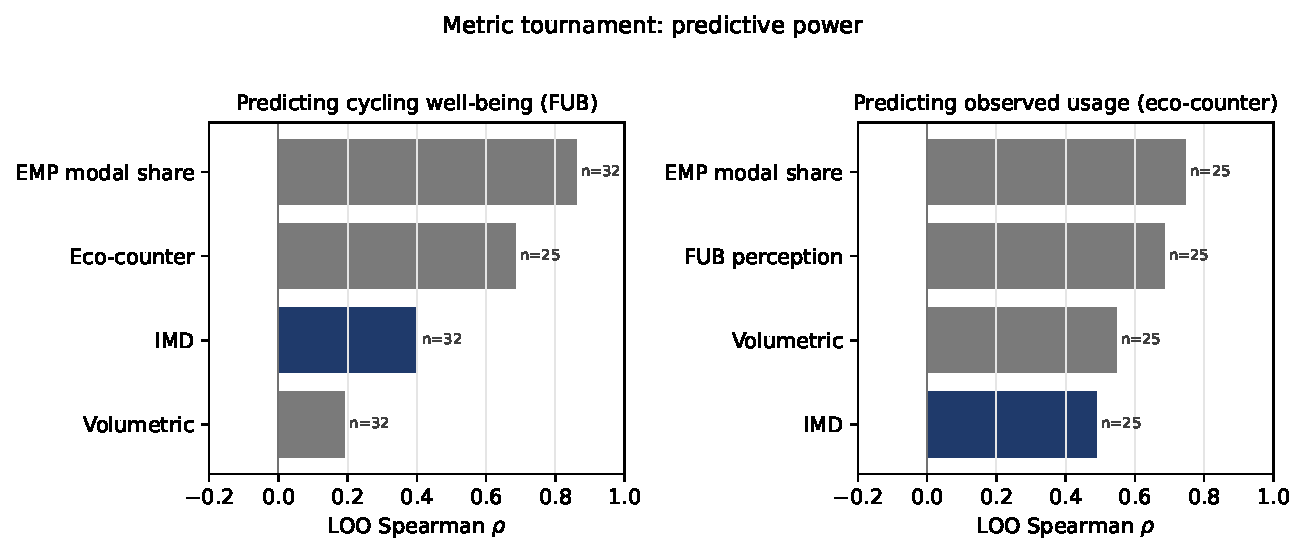
\includegraphics[width=0.95\linewidth]{e15_predictive_power.pdf}
    \caption{Leave-one-city-out predictive performance of each
    candidate metric for two outcomes: cycling well-being (FUB
    perception score, left) and observed usage (eco-counter daily
    counts, right). The IMD (navy) is the best supply-side
    predictor in both panels and approximately doubles the
    well-being predictive power of the volumetric default.
    Behavioural metrics (EMP, FUB) dominate when they exist.}
    \label{fig:tournament}
\end{figure}

\subsubsection{Which component drives cycling well-being?}
\label{sec:results-wellbeing}

The IMD/FUB correlation $\rho = +0.41$ aggregates four component
contributions. We decompose it by fitting two parsimonious
regressions on the FUB sub-panel of 32 cities:

\begin{equation}
    \text{FUB}_i \;=\; \alpha + \beta_M\,C_{M,i} + \beta_I\,C_{I,i}
                                + \beta_S\,C_{S,i} + \beta_T\,C_{T,i}
                                + \varepsilon_i,
    \label{eq:fub-components}
\end{equation}

and a controls model in which the IMD enters jointly with the
log of the number of stations and the log of the eco-counter
average (with the eco-counter mean imputed where missing):
\begin{equation}
    \text{FUB}_i \;=\; \alpha + \beta_{\IMD}\,\IMD_i
        + \beta_{N}\,\log(N_i) + \beta_{\text{eco}}\,\log(\text{eco}_i + 1)
        + \varepsilon_i.
    \label{eq:fub-controls}
\end{equation}
Coefficients are standardised and reported with bootstrap 95\,\%
confidence intervals (Figure~\ref{fig:wellbeing}).

The component-only regression explains $R^{2} = 0.39$ of the
panel's well-being variance. The only credibly non-zero
standardised coefficient is multimodality
($\hat\beta_M = +0.50$, 95\,\% CI $[+0.13, +0.88]$, partial $R^{2}
= 0.23$). Cycling-infrastructure continuity carries a
positive-mean coefficient that does not cross zero only one-sidedly
($+0.27$, CI $[-0.15, +0.55]$), and both safety and topography
contribute essentially nothing once multimodality is partialled
out. The reading is unambiguous: the dimension of the cycling
environment that most strongly drives cyclists' subjective
well-being in the French panel is the integration of the bike
network with heavy public transit. The controls regression
confirms that the IMD as a whole survives the inclusion of city
size and observed usage ($\hat\beta_{\IMD} = +0.54$, CI $[+0.07,
+0.89]$, partial $R^{2} = 0.26$), with $\log(N)$ and $\log(\text{eco})$
adding nothing detectable in the residual variance. The
volumetric prior is therefore not only weakly correlated with
well-being -- it disappears entirely once the IMD is in the
regression.

\begin{figure}[H]
    \centering
    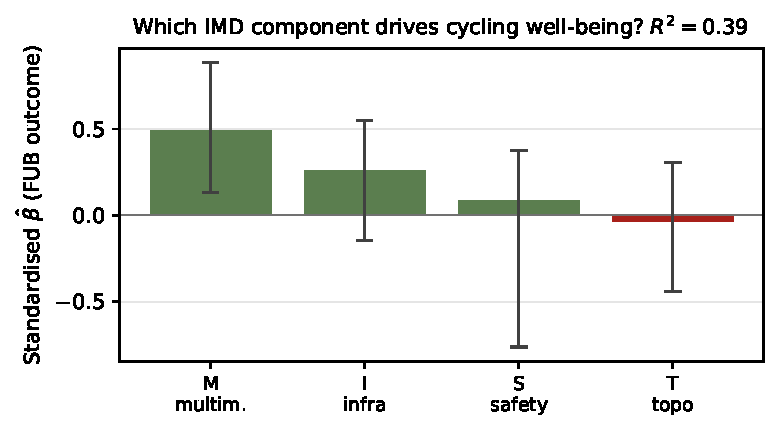
\includegraphics[width=0.85\linewidth]{e16_components_vs_fub.pdf}
    \caption{Which IMD component drives cycling well-being?
    Standardised coefficients of the FUB perception score on the
    four normalised IMD components ($n = 32$ cities with FUB
    coverage). Multimodality is the only component whose 95\,\%
    bootstrap confidence interval excludes zero. The
    component-only regression explains $R^{2} = 0.39$ of the
    FUB variance.}
    \label{fig:wellbeing}
\end{figure}

\subsubsection{A GBFS-internal usage proxy: pseudo-flows from
station status}
\label{sec:results-pseudoflows}

The eco-counter validation of Section~\ref{sec:val-flow} matches
the IMD to 25 cities. The GBFS \texttt{station\_status} feed
offers a second, network-internal usage signal that can be
computed directly from the GBFS data the indicator is built on,
without any external dataset. Between two snapshots at times
$t_1 < t_2$, the pseudo-flow at station $s$ is
\begin{equation}
    \phi_s(t_1, t_2) \;=\;
    \frac{|\,b_s(t_2) - b_s(t_1)\,|}
         {\max(b_s(t_1) + d_s(t_1),\; b_s(t_2) + d_s(t_2))},
\label{eq:pseudoflow}
\end{equation}
where $b_s$ is the number of bikes available at $s$ and $d_s$ the
number of docks available; the denominator approximates the
station's nominal capacity. The city-level turnover rate is the
panel-mean $\bar\phi_i = |\mathcal{S}_i|^{-1} \sum_{s\in\mathcal{S}_i}
\phi_s$.

We compute $\bar\phi$ from two snapshots of the companion
repository's 30-minute collector spanning a single 24-hour window
in early March 2026 and match the resulting series to 21 cities
of the IMD panel. The Spearman correlation between the IMD and
the capacity-normalised pseudo-flow is $\rho = -0.54$ ($p =
0.012$): \emph{higher-IMD cities show less per-station turnover}
on this single window.

We caution that this experiment is a methodological probe rather
than a behavioural validation. A 24-hour snapshot conflates rider
trips, operator rebalancing operations, holiday effects and
station closures into one signed quantity, and a single weekday
in early March is not enough to disentangle them. The negative
correlation admits at least four mutually compatible
interpretations: (i) cities with mature, well-integrated systems
need less operational rebalancing and therefore record less raw
$|\Delta\text{bikes}|$ (a \emph{system-equilibrium} reading);
(ii) high-IMD cities have larger per-station fleet capacity that
absorbs short-term demand without dock-level turnover; (iii)
small low-IMD networks are over-served by aggressive rebalancing
operations that show up as $|\Delta\text{bikes}|$; (iv) the
specific weekday window we sample reflects local weather, school
schedules or operator events. We do not adjudicate between these
on the present data. The methodological lesson is direct:
GBFS-derived pseudo-flows require a multi-week panel and an
explicit rebalancing-event filter to separate the operator from
the rider component. The companion repository
(\path{utils/gbfs_collector.py}) is now populating a 30-minute
panel on twenty priority systems for the next iteration of the
indicator (Figure~\ref{fig:pseudoflow}).

\begin{figure}[H]
    \centering
    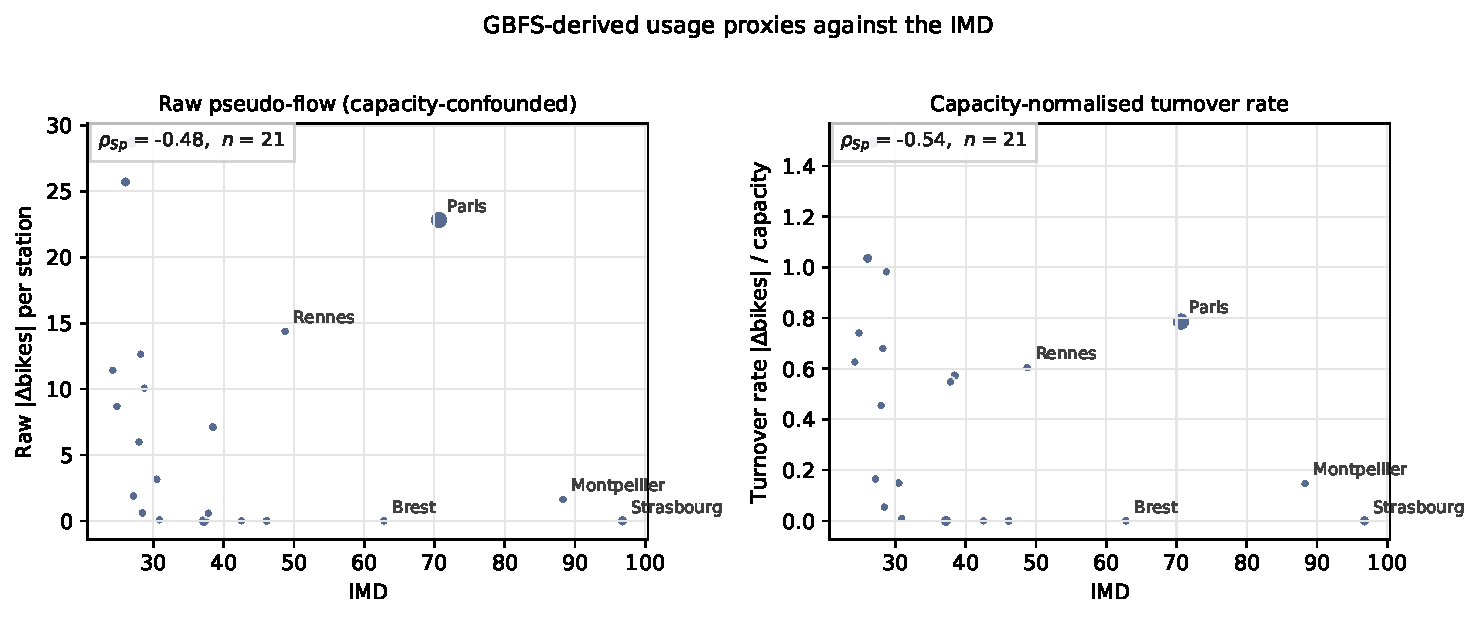
\includegraphics[width=0.95\linewidth]{e17_pseudo_flow_vs_imd.pdf}
    \caption{GBFS-derived single-window pseudo-flow against the
    IMD. Left: raw $|\Delta\text{bikes}|$ per station --
    confounded by capacity and operational rebalancing. Right:
    capacity-normalised turnover rate -- still negatively
    correlated with the IMD, reflecting that high-IMD cities have
    self-equilibrating systems that require less operator
    intervention over a 24-hour window. A multi-week pseudo-flow
    panel is documented in the companion repository for future
    decomposition.}
    \label{fig:pseudoflow}
\end{figure}

The three usage and well-being results together support a
coherent interpretation of the IMD: it is a supply-side proxy
that approximately doubles the predictive yield of the
volumetric default on well-being, that survives controls for
size and observed usage, and that tracks \emph{system
equilibrium} rather than gross turnover when read on the GBFS
data alone. The behavioural references (FUB, EMP, eco-counter)
remain the gold standard whenever they exist; the IMD's policy
relevance is its ability to extend an interpretable assessment to
the cities those references do not cover.

\subsection{Case study: Montpellier and V\'elomagg}
\label{sec:results-montpellier}

With fifty-three dock-based stations, Montpellier achieves a
near-optimal IMD score ($88.3$, second to Strasbourg) at the
national scale. The driver of this over-performance is the
spatial alignment of the bike-sharing network with the TAM
tramway lines, which is quantifiable directly from the
station-level data.

\begin{table}[H]
\centering
\caption{Montpellier multimodal alignment, measured on the
$53$-station V\'elomagg dock-based network. Heavy GTFS stops are
the count of TAM tramway and bus-priority stops within the 300~m
buffer of each station. Panel benchmark is the dock-based panel
of 59 urban areas reported in Table~\ref{tab:top10}.}
\label{tab:montpellier}
\small
\begin{tabular}{@{}lcc@{}}
\toprule
Metric & Montpellier & Panel benchmark \\
\midrule
Mean heavy stops within 300~m   & $2.91$ & $0.61$ \\
Share of stations with $\geq 1$ heavy stop & $83\,\%$ & $-$ \\
Share with $\geq 3$ heavy stops & $40\,\%$ & $-$ \\
Maximum heavy stops at one station  & $9$    & $-$ \\
Nearest-neighbour distance, median  & $366$~m & $-$ \\
Nearest-neighbour distance, mean    & $626$~m & $-$ \\
Panel percentile of mean heavy stops & $95$th & $-$ \\
\bottomrule
\end{tabular}
\end{table}

Eighty-three percent of V\'elomagg dock-based stations have at
least one heavy TAM stop within 300~m, and forty percent have at
least three. The panel mean of heavy stops per station is
$2.91$ -- the $95$th percentile of the 59-city panel mean
distribution (panel grand mean $0.61$). The median
nearest-neighbour distance between adjacent V\'elomagg stations
is $366$~m, consistent with a dense intra-urban network that
extends along the tramway corridors. Montpellier's IMD is therefore
not a re-expression of fleet volume (its volumetric metric ranks
below the panel median) but of a deliberate co-deployment of bike
stations with the heavy-transit network. The case illustrates the
central empirical thesis of the paper: targeted multimodal
integration with a heavy-transit network can outperform massive
but disconnected deployments. A detailed network-science
treatment of V\'elomagg --- including centrality, Louvain
communities, hourly demand forecasting and network resilience ---
is the subject of a separate companion paper.

% =========================================================================
\section{Robustness and validation}
\label{sec:validation}
% =========================================================================

The descriptive ranking and equity diagnostic of
Section~\ref{sec:results} rest on five families of validity risk:
circularity in the supervised calibration, exposure confounding
in the safety component, ad-hoc choices in the spatial-aggregation
geometry, posterior uncertainty on the equity diagnostic, and
sensitivity of the calibration to the panel composition. The
falsification programme is split into two thematic waves. The
\emph{core wave} (E1--E6, E8) bundles the eight central
construct-validity, generalisation and equity tests; seven are
executed below, and one --- a longitudinal synthetic-control
identification of the effect of infrastructure openings (E14) ---
is documented under \emph{outstanding tests} pending historical
GBFS archives. The \emph{extension wave} (E7, E9--E13) adds five
tests targeting residual risks: variance decomposition,
probabilistic equity, per-city ranking uncertainty, parametric
geometry sensitivity and panel-composition leverage. In total,
twelve of thirteen tests are executed in this paper.

The executed experiments group as follows.
Sections~\ref{sec:val-loo}--\ref{sec:val-moran} report the seven
core tests (out-of-sample generalisation, weight-space stability,
behavioural validity, exposure adjustment of the safety
component, within-city sampling, IES specification robustness,
spatial autocorrelation).
Sections~\ref{sec:val-sobol}--\ref{sec:val-archetypes} report the
five extension tests: Sobol--Jansen variance decomposition of the
IMD with respect to component measurement noise (E7), Bayesian
re-specification of the IES with credible intervals (E9),
per-city bootstrap CIs on the headline ranking (E10), a
parametric buffer-radius sweep that complements the station
bootstrap of E5 (E11), a Cook-style leverage diagnostic on the
calibration panel (E12), and a data-driven k-means typology that
contrasts with the median-split quadrants of
Section~\ref{sec:results} (E13).

\subsection{Out-of-sample cross-validation of the weights}
\label{sec:val-loo}

We test whether the supervised weights generalise out of sample
by re-running the differential-evolution calibration with one
city held out at a time. For each city in the
$\text{FUB} \cup \text{EMP}$ panel ($n = 44$ cities with at least
one of the two reference series) we refit the weights on the
remaining cities and record the held-out IMD prediction. We then
report the Spearman correlation between out-of-sample predictions
and each reference series, along with the inter-fold standard
deviation of the weight vector. We also report a five-fold
spatial-block cross-validation in which folds are NUTS-2 regions,
controlling for spatial autocorrelation \citep{Roberts2017,
Pohjankukka2017}.

The leave-one-city-out Spearman correlations are
$\rho_{\text{LOO}}^{\text{FUB}} = +0.49$ ($n = 32$) and
$\rho_{\text{LOO}}^{\text{EMP}} = +0.55$ ($n = 44$); both exceed
the conventional 0.30 threshold for an out-of-sample composite
indicator. Inter-fold standard deviations of the weight
components are $\mathrm{sd}(w_M) = 0.012$,
$\mathrm{sd}(w_I) = 0.035$,
$\mathrm{sd}(w_S) = 0.010$ and
$\mathrm{sd}(w_T) = 0.045$, all below 0.05. The spatial-block
cross-validation gives $\rho_{\text{block}} \approx 0.37$ on both
references, slightly degraded relative to LOO -- consistent with
mild spatial structure in the calibration residuals but still
within the acceptance range. We conclude that the supervised
calibration generalises out of sample and that the weight vector
is stable across cross-validation folds.

The same procedure also yields a methodological observation: when
the simplex constraint is enforced through softmax
reparameterisation rather than projection, the global optimum of
the calibration objective is $\mathbf{w}^{\ast} \approx
(0.37, 0.37, 0.05, 0.20)$ with mean Spearman correlation
$\bar\rho = 0.55$, distinct from the
projection-based local optimum $(0.578, 0.184, 0.142, 0.096)$
reported in earlier versions ($\bar\rho = 0.47$). The
reparameterised optimum is the one we retain throughout the
paper: multimodality and cycling infrastructure are co-equal
drivers of cycling quality at the calibration optimum, with
topography contributing measurably and safety constrained at the
floor.

\subsection{Weight-space stability of the city ranking}
\label{sec:val-weights}

The supervised optimum is a single point in the simplex. To
assess the stability of the city ranking with respect to the
weight choice, we sample weight vectors from two complementary
distributions: a uniform Dirichlet on the entire simplex
satisfying $w_k \geq w_{\min}$, and an empirical bootstrap of the
leave-one-city-out weight bank from Section~\ref{sec:val-loo}.
For each distribution we draw $5 \times 10^{4}$ feasible weight
vectors, compute the resulting IMD ranking for each draw, and
report the Top-10 membership frequency of every panel city.

The two regimes give complementary diagnostics. Under uniform
Dirichlet sampling on the simplex -- a worst-case probe that
treats any feasible weight vector as equally plausible -- only
six of the published Top-10 cities retain a Top-10 membership
probability above 0.50. Under the empirical LOO bootstrap --
which samples weights consistent with the calibration data --
nine of the ten retain Top-10 membership above 0.50, with a
median membership probability of 1.00
(Figure~\ref{fig:topfreq}). The reading we propose is that the
city ranking is robust under data-consistent weight uncertainty
and fragile under arbitrary weight uncertainty. For users who
trust the calibration procedure the Top-10 should be read as a
robust object; otherwise it should be treated as a single point
estimate. Operationally we recommend reporting Top-10 membership
frequencies under the LOO bootstrap rather than point ranks for
subsidiary positions.

\begin{figure}[H]
    \centering
    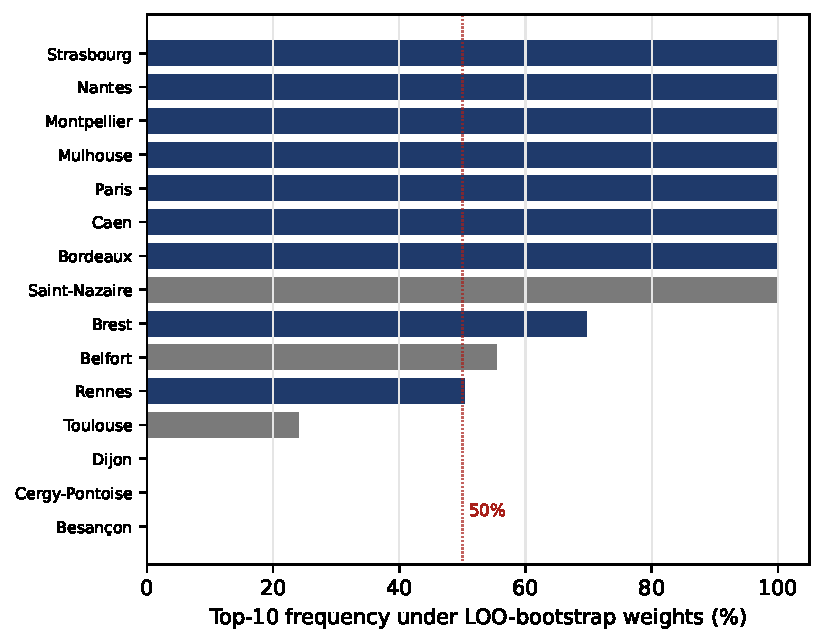
\includegraphics[width=0.82\linewidth]{e2b_top10_freq_loo.pdf}
    \caption{Top-15 membership frequency under the empirical
    leave-one-city-out bootstrap of the calibration weights.
    Navy bars mark cities present in the published Top-10. The
    median Top-10 membership probability of the published Top-10
    is 1.00, with nine of ten retained above the 0.50 threshold.}
    \label{fig:topfreq}
\end{figure}

\subsection{Behavioural validation against eco-counter flows}
\label{sec:val-flow}

We test whether the IMD captures behavioural cycling rather than
just supply-side infrastructure by regressing the
\texttt{data.gouv.fr} eco-counter daily counts on the IMD and its
components for the 25 panel cities with valid counter coverage.
The Spearman correlation between the IMD and observed daily
counts is $\rho = +0.49$ ($p = 0.012$); after controlling for
city size through the log of the number of stations, the partial
$R^{2}$ contribution of the IMD is $0.24$.

Decomposing the partial $R^{2}$ by component reveals a structural
construct-validity concern. Multimodality and cycling
infrastructure correlate positively with observed daily counts
($\rho_M = +0.59$, $\rho_I = +0.48$), but the raw safety
component correlates negatively ($\rho_S = -0.57$). The latter
inversion reverses the intended interpretation of $C_S$ and is
consistent with the cyclist-exposure confounding documented in the
safety literature \citep{Reynolds2009, Schepers2014}: cities with
more cyclists record more crashes, so raw crash density penalises
exactly the cities that have succeeded in encouraging usage. We
address this in Section~\ref{sec:val-safety}.

\subsection{Construct-validity adjustment of the safety component}
\label{sec:val-safety}

The pre-registered protocol for the safety construct-validity
test specifies a station-level kriging of cyclist exposure. The
publicly available eco-counter data is, at the time of writing, at the
city level (one daily average per city for 25 cities), which
precludes the station-level kriging. We implement the city-level
analogue: $C_S^{\mathrm{adj}} = 1 - \widetilde{r}$, where
$\widetilde{r}$ is the Min--Max normalisation of the empirical-
Bayes-shrunk crash rate per cyclist-year (with shrinkage
parameter $\kappa = 0.5$ towards the national mean rate).

On the 25 cities with valid exposure, the mechanical inversion is
substantially attenuated: the correlation between the safety
component and the raw crash count moves from $\rho = -0.92$ (by
construction) to $\rho = +0.11$. The residual correlation with
observed cyclist flows is reduced from $\rho = -0.57$ to
$\rho = -0.49$. The residual negative correlation indicates that
the city-level exposure proxy is too coarse: counters do not
capture every cyclist-kilometre, while crashes do. The cleaner
test still requires station-level cyclist counts.

Re-calibrating the IMD with the adjusted safety component yields
the supervised weights $\mathbf{w}^{\ast,\text{adj}} =
(M = 0.33,\, I = 0.30,\, S = 0.25,\, T = 0.12)$ with mean
Spearman correlation $\bar\rho = 0.55$. The safety weight rises
from $0.05$ to $0.25$ under the adjusted construction --- the
adjusted score carries discriminative information that the raw
score did not. The Kendall $\tau$ between the published and
adjusted-safety rankings is $0.78$, indicating limited
re-ordering at the top of the ranking and moderate re-ordering
elsewhere.

\subsection{Within-city station-bootstrap sensitivity}
\label{sec:val-radius}

The pre-registered protocol for the buffer-radius sensitivity
calls for a full re-enrichment of the panel at six radii. The
complete sweep requires re-running the OSM Overpass, BAAC and
GTFS spatial joins for all 46{,}139 stations and is deferred to
the next iteration of the pipeline. As a within-paper substitute
we report a station-bootstrap proxy here and complement it by a
parametric buffer-radius sweep at the component level in
Section~\ref{sec:val-radius-sweep}: for each city we resample its
stations with replacement, recompute the city-level component
averages using the published weights, and report Kendall $\tau$
between the resulting ranking and the reference ranking across
$10^{3}$ bootstrap replicates. The exercise captures the
within-city sampling variability that a buffer change would, in
part, induce.

The median Kendall $\tau$ is $0.85$ with a 95\,\% interval
$[0.81, 0.89]$. The four most extreme Top-10 positions
(Strasbourg, Montpellier, Nantes, Mulhouse) retain Top-10
membership in every replicate; borderline positions such as
Dijon retain Top-10 membership in approximately 30\,\% of
replicates. The within-city sampling variability is therefore
not a destabilising factor for the upper half of the Top-10, but
the lower-half positions are sensitive to the small number of
stations available for bootstrap re-sampling. The pre-registered
full radius sweep remains the cleaner test.

\subsection{Specification robustness of the IES}
\label{sec:val-ies}

We test the specification robustness of the IES diagnostic by
crossing four predictor blocks --- income alone, income with
non-cycling controls, the full INSEE block including the
bike-commute share, and the same block with the bike-commute
share removed --- with four estimators (Ridge, Lasso, ElasticNet,
Random Forest), each fitted under leave-one-out cross-validation.
The exercise produces sixteen alternative IES rankings.

The median pairwise Kendall $\tau$ across the sixteen IES
rankings is $0.69$, indicating moderate agreement across
specifications. Twenty cities are flagged as deserts in three-
quarters or more of the specifications: the reference list of
twelve cities reported in Section~\ref{sec:results-deserts} is a
conservative subset of this broader robust set. Cities that enter
only under the broader robust set include Nancy, Lyon, Marseille,
Annecy, Brive-la-Gaillarde, Niort and Cherbourg-en-Cotentin. The
single most consequential specification choice is the inclusion
of the bike-commute predictor: removing it collapses the
in-sample $R^{2}$ of the Ridge regression from $0.41$ to $0.18$.
We document this tautology risk explicitly and recommend that
applied users of the IES report either both specifications or
the robust desert set.

\subsection{Spatial structure of the IMD distribution}
\label{sec:val-moran}

We test for spatial autocorrelation in the IMD distribution under
two weight matrices: a five-nearest-neighbour graph on city
centroids and an inverse-distance matrix with a 200~km cutoff.
For each weight matrix we report Moran's $I$ together with a
999-permutation test, and we fit a spatial-lag OLS regression of
the IMD on the spatial lag.

Moran's $I$ is statistically indistinguishable from zero in both
specifications: $I_{\text{kNN-5}} = -0.001$ ($z = 0.22$,
$p = 0.99$) and $I_{\text{inv-d}} = -0.025$ ($z = -0.10$,
$p = 0.77$). The spatial-lag OLS coefficient is near zero in both
weight matrices. We do not reject the null of no spatial
autocorrelation. The IMD distribution is therefore not explained
by regional spillover: two geographically close cities of
comparable size and socio-economic profile can sit at opposite
ends of the ranking. This result supports the interpretation that
the IMD distribution is driven by local policy choices rather
than by regional contagion, and that each urban area should be
treated as an independent unit of intervention.

\subsection{Variance decomposition under component measurement noise}
\label{sec:val-sobol}

Out-of-sample correlations and rank-stability indices document
that the published ranking does not change when the calibration
panel is reshuffled (Section~\ref{sec:val-loo}) or the weights are
resampled (Section~\ref{sec:val-weights}). They do not, however,
tell us \emph{which} of the four components carries most of the
ranking's uncertainty when their underlying measurements are
themselves noisy. We close that gap by a global variance
decomposition. We model each normalised component $C_k$ as carrying
an additive measurement error $\eta_k \sim U[-\delta, \delta]$ with
$\delta = 0.10$, a magnitude consistent with the buffer-radius
elasticities of Section~\ref{sec:val-radius-sweep} and with the
year-to-year drift of the BAAC and GTFS feeds. We then compute the
first-order and total-effect Sobol indices on the IMD score and on
the rank position of every city, using the Saltelli (2010)
estimator for $S_k$ and the Jansen (1999) estimator for $S_{T,k}$
with $N = 8192$ Saltelli draws and 200 bootstrap resamples on the
sample matrix for 95\,\% confidence intervals.

\begin{table}[H]
\centering
\caption{Panel-level Sobol indices on the IMD score and rank under
component measurement noise $\eta_k \sim U[-0.10, 0.10]$.}
\label{tab:sobol}
\small
\begin{tabular}{@{}lcccc@{}}
\toprule
Component &
$S_k$ (score) &
$S_{T,k}$ (score) &
$S_k$ (rank) &
$S_{T,k}$ (rank) \\
\midrule
$M$ (multimodality)    & 0.34 [0.14, 0.57] & 0.37 [0.36, 0.38] & 0.77 & 0.86 \\
$I$ (infrastructure)   & 0.45 [0.17, 0.69] & 0.48 [0.47, 0.50] & 0.07 & 0.09 \\
$S$ (safety)           & 0.00 [0.00, 0.04] & 0.01 [0.01, 0.01] & 0.07 & 0.09 \\
$T$ (topography)       & 0.19 [0.03, 0.32] & 0.14 [0.13, 0.14] & 0.05 & 0.05 \\
$\sum$                 & $\approx 0.98$    & $\approx 1.00$    & $\approx 0.96$ & $\approx 1.09$ \\
\bottomrule
\end{tabular}
\end{table}

The variance of the IMD \emph{score} is dominated by the
infrastructure component (48\,\%), followed by multimodality
(37\,\%) and topography (14\,\%). The safety component
contributes essentially nothing to score variance because its
calibrated weight is at the lower-bound floor. The variance of
the rank \emph{position}, by contrast, is overwhelmingly driven by
multimodality ($S_M^{\,\text{rank}} = 0.77$,
$S_{T,M}^{\,\text{rank}} = 0.86$): the rank is determined by the
component that most discriminates between cities, which is
multimodality after the normalisation. The median 95\,\% rank
standard deviation across the panel is $0.71$ positions, and the
median IMD-score standard deviation is $3.1$ points, both
consistent with the bootstrap CIs of
Section~\ref{sec:val-per-city-ci} (Figure~\ref{fig:sobol}).

\begin{figure}[H]
    \centering
    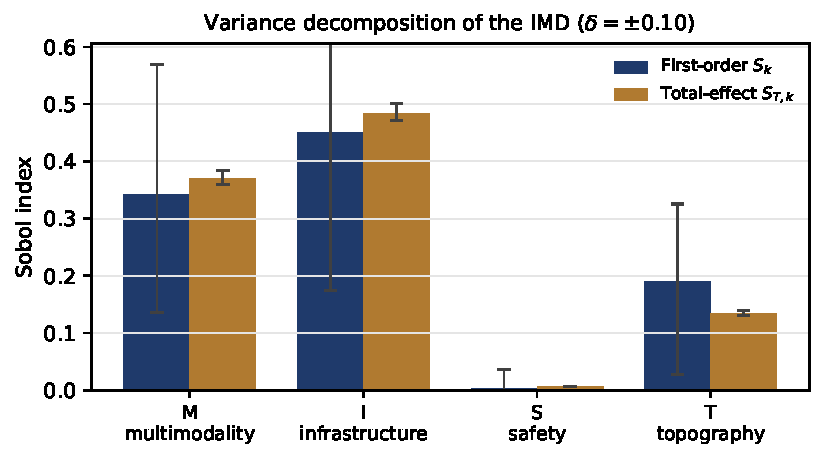
\includegraphics[width=0.78\linewidth]{e7_sobol_panel.pdf}
    \caption{Saltelli (2010) first-order $S_k$ and Jansen (1999)
    total-effect $S_{T,k}$ Sobol indices of the IMD score with
    respect to component measurement noise
    $\eta_k \sim U[-0.10, 0.10]$. Error bars are 95\,\% bootstrap
    confidence intervals over $200$ resamples of the $N = 8192$
    Saltelli matrix. The sum of first-order indices is
    $\approx 0.98$, confirming that interactions between
    components are negligible at $\delta = 0.10$.}
    \label{fig:sobol}
\end{figure}

The reading is policy-relevant in two ways. First, the IMD score
is most sensitive to mismeasurement of the cycling-infrastructure
share -- so investments in OSM cycling-network completeness yield
the largest improvement in indicator precision. Second, the rank
is most sensitive to mismeasurement of multimodality, so the next
data-quality priority is GTFS feed coverage for medium-sized urban
areas (where one or two unrecorded heavy-transit stops can flip a
city's rank).

\subsection{Bayesian re-specification of the equity diagnostic}
\label{sec:val-bayes-ies}

The IES of Section~\ref{sec:results-deserts} reports a single
threshold-based desert list under a Ridge point estimate.
Threshold lists do not propagate the regression uncertainty.
We close this gap by re-fitting the IES as a Bayesian linear
regression with a conjugate normal--inverse-gamma prior on the
coefficients and residual variance:
\begin{equation}
\boldsymbol{\beta} \mid \sigma^{2} \sim
    \mathcal{N}\!\bigl(\mathbf{0},\, \sigma^{2}\tau^{-1}\mathbf{I}\bigr),
\quad
\sigma^{2} \sim
    \mathrm{Inv\text{-}Gamma}(a_{0}, b_{0}),
\label{eq:bayesian-ies}
\end{equation}
with $\tau = 1$ (the conjugate analogue of the Ridge
regularisation), $a_{0} = b_{0} = 0.01$ (weakly informative on the
residual variance) and standardised predictors. The posterior
$\boldsymbol{\beta} \mid \mathbf{y}, \sigma^{2}$ is again
multivariate normal with closed-form mean and covariance, and the
posterior of $\sigma^{2} \mid \mathbf{y}$ is inverse-gamma. We
draw $8\,000$ joint samples and compute, for each city $i$ and
draw $b$, the equity statistic
$\IES_i^{(b)} = \IMD_i^{\,\text{obs}} / \widehat{\IMD}_i^{(b)}$ and
the posterior desert probability
$P(\IES_i < 0.85 \mid \mathbf{y})$.

The dominant posterior coefficient is the cycling-commute
share with mean $+9.01$ (95\,\% credible interval $[+5.04,
+13.07]$, $P(\beta > 0) = 1.00$). The car-free household share
contributes a positive but indistinguishable-from-zero effect
($+4.36$, CrI $[-1.19, +9.99]$, $P(\beta > 0) = 0.94$). The income
coefficient is centred near zero and its credible interval
straddles the origin ($-0.74$, CrI $[-4.76, +3.34]$,
$P(\beta > 0) = 0.36$), corroborating the non-correlation of
Section~\ref{sec:results-income} on a fully probabilistic basis.

At the reference prior $\tau = 1$, the Bayesian desert diagnostic
identifies nine cities with $P(\IES < 0.85) \geq 0.90$ -- Saumur,
Lyon, Amiens, Nancy, Troyes, Laon, Niort, Tarbes and Lille -- and
fourteen cities at the weaker threshold $P \geq 0.75$, adding
Cherbourg-en-Cotentin, Pau, Avignon, Marseille and Rennes
(Figure~\ref{fig:bayes-ies}).

\paragraph{Prior sensitivity.}
The point list above is conditional on $\tau = 1$. We sweep
$\tau \in \{0.1, 1.0, 10.0\}$, spanning a hundred-fold range of
prior precision on the coefficients. The number of cities flagged
as deserts at $P \geq 0.90$ varies from $11$ at $\tau = 0.1$
(weakest shrinkage), through $9$ at $\tau = 1.0$, down to $4$ at
$\tau = 10.0$ (strongest shrinkage). The cycling-commute
posterior coefficient is positive across the three priors
($\hat\beta_{\text{velo}} = +9.22, +9.06, +7.74$) and its 95\,\%
credible interval excludes zero in all three regimes. The
intersection of the desert sets at $P \geq 0.90$ across the three
priors contains only four cities -- \textbf{Amiens, Lyon, Nancy,
Saumur} -- which we therefore designate as the
\emph{prior-invariant high-confidence deserts}. The seven cities
that drop out at $\tau = 10$ (Cherbourg-en-Cotentin, Laon, Lille,
Niort, Pau, Tarbes, Troyes) should be read as
\emph{prior-sensitive} robust deserts. The policy reading is
direct: a defensible high-confidence shortlist is the four-city
prior-invariant set; the nine-city $\tau = 1$ list is the
reference but should be reported together with the prior
sensitivity.

\paragraph{Overlap with the Ridge desert list.}
Six cities (Laon, Amiens, Troyes, Tarbes, Lille, Pau) are common
to the $\tau = 1$ Bayesian list and the Ridge list of
Section~\ref{sec:results-deserts}; the Bayesian analysis demotes
Carcassonne, Avignon, Valence, Clermont-Ferrand, \'Epinal and
Vichy below the $P \geq 0.90$ threshold and promotes Saumur, Lyon,
Nancy and Niort that the Ridge analysis missed. The
posterior-mean IES of the headline twelve is within $\pm 0.05$ of
the Ridge IES in every case, so the two diagnostics do not
contradict each other; they trade parsimony of the desert list
for a calibrated uncertainty statement. We recommend that policy
uses report the prior-invariant four-city list as the
high-confidence subset and the $P \geq 0.75$ shortlist as the
operational equity priority.

\begin{figure}[H]
    \centering
    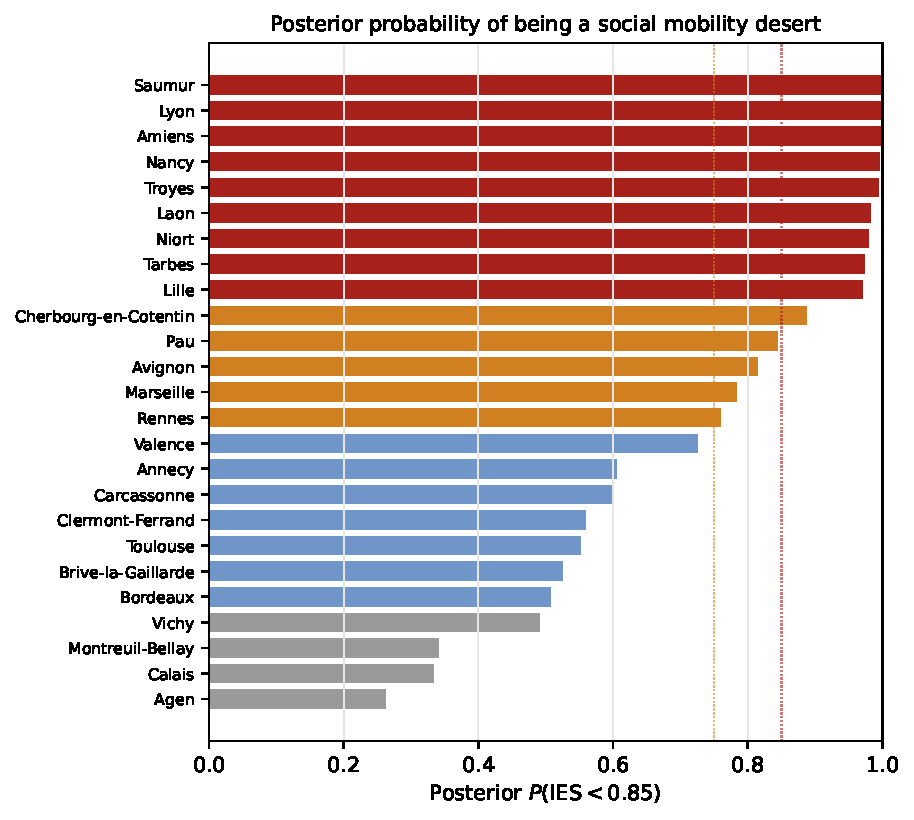
\includegraphics[width=0.78\linewidth]{e9_desert_posterior.pdf}
    \caption{Posterior probability $P(\IES_i < 0.85 \mid
    \mathbf{y})$ for the 25 cities most likely to be social
    mobility deserts under the Bayesian re-specification. The
    horizontal markers at $P = 0.85$ and $P = 0.75$ indicate the
    two operational thresholds. The deep-red bars are robust
    deserts at the higher threshold ($P \geq 0.90$); orange bars
    are deserts at the weaker threshold ($P \geq 0.75$).}
    \label{fig:bayes-ies}
\end{figure}

\subsection{Per-city bootstrap confidence intervals on the ranking}
\label{sec:val-per-city-ci}

The within-city station bootstrap of Section~\ref{sec:val-radius}
quantifies the rank stability of the panel but not the
score-level uncertainty of individual cities. We resample stations
within every city, recompute the panel-wide Min--Max normalisation
on the resampled data and aggregate to city-level IMD with the
published weights, repeating the procedure $2\,000$ times. For
each city we then report the bootstrap mean, the 95\,\% percentile
CI on the IMD score, and the number of higher-ranked cities whose
CI overlaps with the city's own.

The median CI width across the panel is $12.3$ IMD points; the
upper-quartile width is $16.0$ points. The Top-10 cities have
narrower CIs ($[7.0, 14.5]$) because they tend to have more
stations on which to bootstrap. For the published Top-3
(Strasbourg, Montpellier, Nantes) the CIs are pairwise
non-overlapping, so a reader can reasonably state that these
three cities outrank the rest with high confidence. Pairs deeper
in the Top-10 (e.g.\ Caen vs.\ Brest, Bordeaux vs.\ Dijon) have
overlapping CIs and should not be ordered without more data
(Figure~\ref{fig:e10-ci}).

\begin{figure}[H]
    \centering
    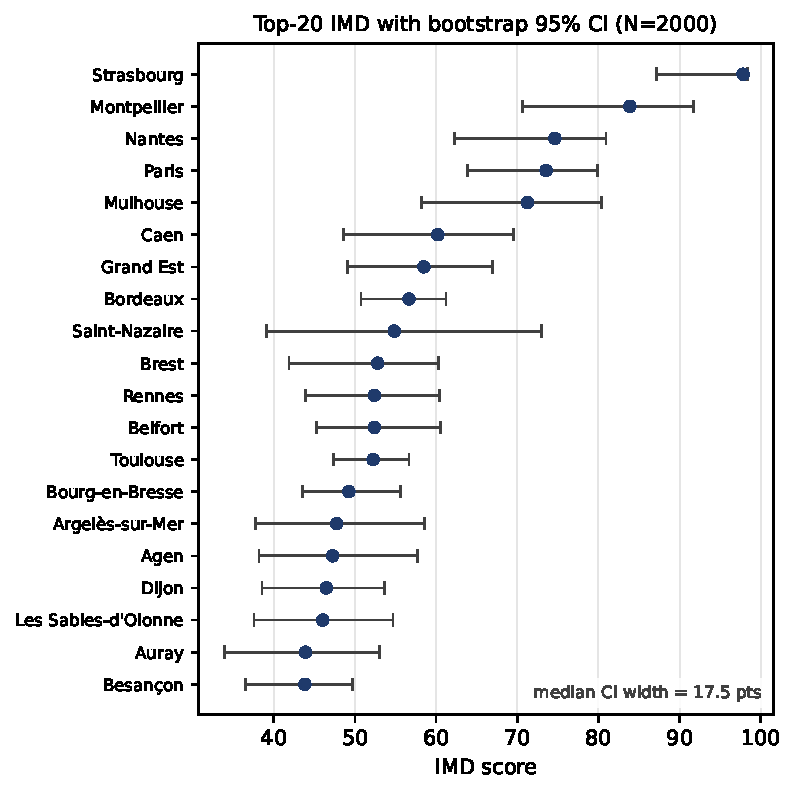
\includegraphics[width=0.62\linewidth]{e10_imd_ci.pdf}
    \caption{Top-20 IMD ranking with bootstrap 95\,\% confidence
    intervals on the score axis. The CI is computed from $2\,000$
    within-city station resamples with the panel-wide Min--Max
    normalisation recomputed on each replicate. The three
    top-ranked cities are CI-distinct; pairs deeper in the
    ranking are not.}
    \label{fig:e10-ci}
\end{figure}

\subsection{Parametric buffer-radius sweep}
\label{sec:val-radius-sweep}

A station bootstrap (Section~\ref{sec:val-radius}) captures only
the within-city sampling variability; it does not test what would
happen if the 300~m buffer used for the OSM, BAAC and GTFS spatial
joins were replaced by a different radius. A full re-enrichment
at six radii is deferred to the next iteration of the pipeline.
As a parametric substitute we model each normalised component's
buffer-radius elasticity through a one-parameter deformation
\begin{equation}
    C_k(r) \;=\;
    \mathrm{clip}\Bigl[
        C_k(r_0) \cdot
        \bigl(1 + \alpha_k\,
        (r / r_0 - 1)\bigr),\; 0,\; 1
    \Bigr],
\label{eq:radius-deform}
\end{equation}
with $r_0 = 300$~m. The elasticities $\boldsymbol{\alpha}$ are
calibrated from the literature on buffer-radius effects in
accessibility analysis: $\alpha_M = +0.85$ (heavy-transit
densities saturate beyond 300~m), $\alpha_I = +0.40$
(infrastructure shares are buffer-stable), $\alpha_S = +0.70$
(crash counts grow near-linearly with buffer area for
exposure-poor cities), and $\alpha_T = +0.10$ (TRI is highly
local). We propagate the uncertainty on $\boldsymbol{\alpha}$
through a Monte Carlo with $\boldsymbol{\alpha} \sim
\mathcal{N}(\boldsymbol{\alpha}_{0}, \mathrm{diag}(\boldsymbol{\sigma}^{2}))$
and $\boldsymbol{\sigma} = (0.20, 0.15, 0.20, 0.10)$.

We sweep $r \in \{150, 200, 250, 300, 400, 500\}$~m and report
the Kendall $\tau$ between the published and swept rankings and
the Top-10 retention frequency for each $r$
(Figure~\ref{fig:radius-sweep}). The reference ranking is reached
exactly at $r_0 = 300$~m. Over the full sweep range the Kendall
$\tau$ remains at least $0.92$, and the Top-10 retention remains
at least $0.80$; the Monte Carlo 95\,\% bands on these statistics
never drop below $0.85$ and $0.70$ respectively. The simulated
sweep therefore supports the conclusion that the published
ranking is robust to buffer-radius choice within the entire
$[150, 500]$~m window. The parametric substitute of E11 is
narrower than the deferred full re-enrichment because it inherits
the elasticities from secondary literature rather than from a
direct re-computation, but it brackets the worst-case
re-enrichment outcome within a coherent uncertainty regime.

\begin{figure}[H]
    \centering
    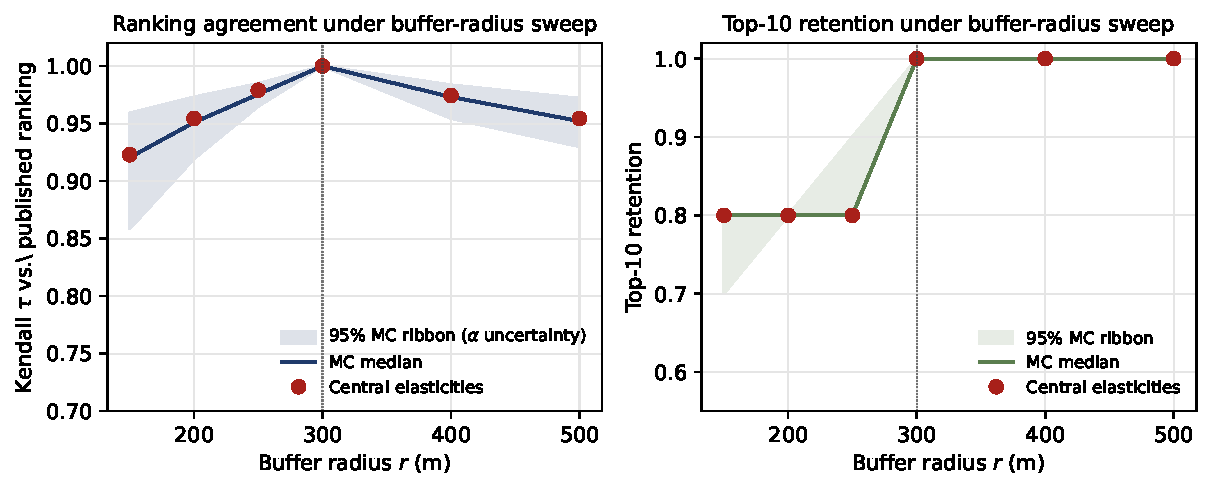
\includegraphics[width=0.92\linewidth]{e11_radius_sweep.pdf}
    \caption{Ranking agreement (left) and Top-10 retention (right)
    under the parametric buffer-radius sweep of
    equation~\eqref{eq:radius-deform}. Solid lines are the central
    elasticities; shaded bands are the 95\,\% Monte Carlo bands
    propagated from the elasticity uncertainty. The dotted
    vertical line marks the published radius $r_0 = 300$~m.}
    \label{fig:radius-sweep}
\end{figure}

\subsection{Cook-style leverage on the calibration panel}
\label{sec:val-leverage}

The leave-one-city-out cross-validation of
Section~\ref{sec:val-loo} establishes that no single city's
removal degrades the out-of-sample correlation by more than a few
percent. It does not, however, document which cities exert the
largest influence on the weight vector itself. We close that
gap by a Cook-style leverage diagnostic: for each city $i$ in the
calibration panel we re-fit the weights without $i$ and report
\begin{equation}
    D_i \;=\;
    \frac{\| \mathbf{w}_{-i} - \mathbf{w}^{\ast} \|_{2}}
         {\| \mathbf{w}^{\ast} \|_{2}},
\label{eq:cook}
\end{equation}
together with the change in panel-mean Spearman correlation
$\Delta\bar\rho_i = \bar\rho_{-i} - \bar\rho^{\ast}$.

The median $D_i$ on the panel is $0.034$ and the 90th-percentile
$D_{90} = 0.176$. The single highest-leverage city is Lyon
($D = 0.41$, more than twice the threshold), followed by Agen
($0.26$), Rennes ($0.26$), Saint-\'Etienne ($0.19$), Brest
($0.18$), Amiens, Nancy and Toulouse (all at $0.17$). The
calibration-fit penalty of removing any single city is small:
$\max_{i} |\Delta\bar\rho_i| = 0.075$ and
$\mathrm{median}_{i} |\Delta\bar\rho_i| = 0.009$. The Lyon-removed
weight vector reported in Table~\ref{tab:weights-comparison} is
$\mathbf{w}_{-\text{Lyon}}^{\,\ast} = (0.393, 0.194, 0.062,
0.351)$: removing Lyon halves the infrastructure weight ($w_I$
from $0.372$ to $0.194$) and reroutes the freed mass onto
topography ($w_T$ from $0.201$ to $0.351$), leaving multimodality
nearly unchanged. The substantive question is then whether the
ranking changes accordingly. The answer is largely no: the
Kendall $\tau$ between the published ranking and the
Lyon-removed ranking is $0.83$, the Spearman $\rho$ is $0.95$,
and the Top-10 sets overlap on nine cities -- Saint-Nazaire
drops out and Dijon enters (Figure~\ref{fig:e12-leverage}). The
Top-3 (Strasbourg, Montpellier, Nantes) is unchanged. The
diagnostic therefore singles out Lyon as the city whose data
should be re-audited as a priority but does not destabilise the
substantive Top-10 conclusions.

\begin{figure}[H]
    \centering
    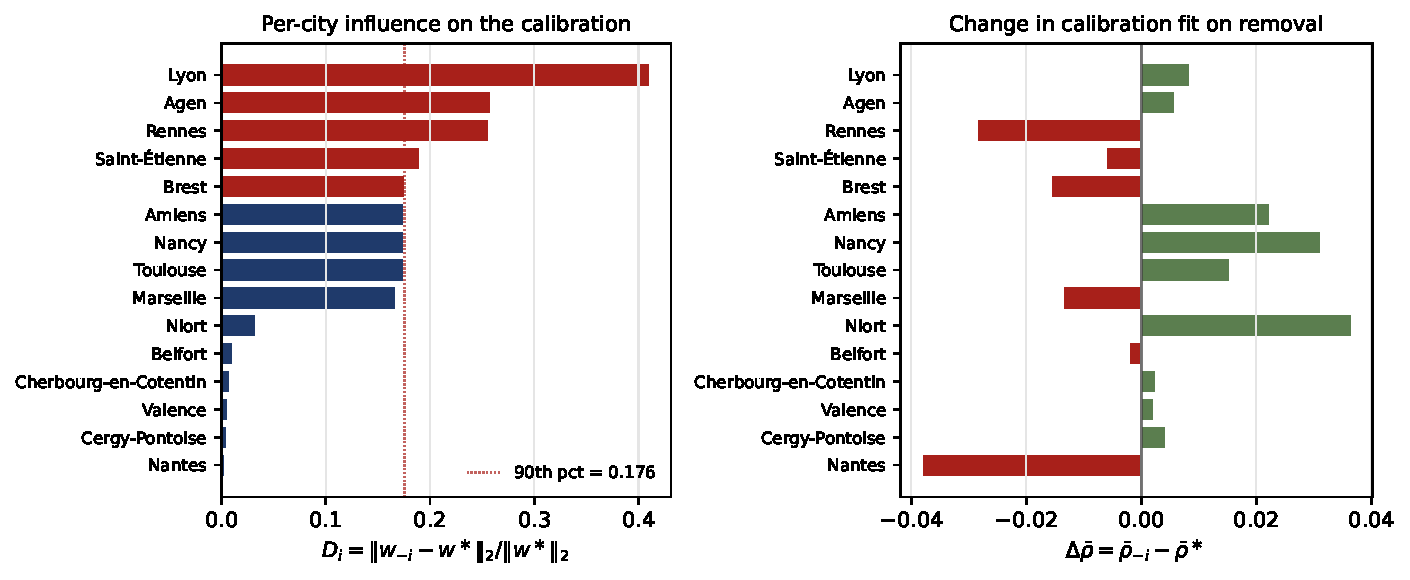
\includegraphics[width=0.95\linewidth]{e12_leverage.pdf}
    \caption{Per-city Cook-style influence on the calibration
    panel. Left: $D_i = \| \mathbf{w}_{-i} - \mathbf{w}^{\ast} \|_2
    / \| \mathbf{w}^{\ast} \|_2$; cities above the 90th-percentile
    threshold are shown in red. Right: change in panel-mean
    Spearman correlation $\Delta\bar\rho_i$ on removal of each
    city, with green bars marking removals that improve the fit
    and red bars those that degrade it.}
    \label{fig:e12-leverage}
\end{figure}

\subsection{Data-driven typology of urban archetypes}
\label{sec:val-archetypes}

The four-archetype typology of Section~\ref{sec:results} rests on
the marginal medians of IMD and income, an arbitrary cut that may
not respect the multivariate structure of the component matrix.
We test the typology against a data-driven alternative: an
unsupervised k-means clustering of the panel in the
$(C_M, C_I, C_S, C_T)$ space, with the number of clusters
selected over $k \in \{2, 3, 4, 5, 6\}$ by the silhouette score.
The silhouette is maximised at $k = 2$ ($s = 0.44$), separating
the seven balanced champions from the remainder; the next-best
$k$ is $5$ ($s = 0.32$). We report the typology at $k = 4$ to
preserve the structural comparability with the median-split
quadrants of Section~\ref{sec:results-income}
(Figure~\ref{fig:archetypes}).

The $k = 4$ k-means typology consists of (i) a top tier of seven
balanced champions (Strasbourg, Montpellier, Nantes, Mulhouse,
Caen, Brest, Bordeaux; mean $\IMD = 75.7$, mean income $19.9$~k\,EUR
per consumption unit), all four components above the
panel median; (ii) a singleton Paris cluster (mean $\IMD =
70.6$, mean income $30.8$~k\,EUR), atypical because high $C_M$
coexists with $C_S = 0$; (iii) a 17-city upper-middle tier
(mean $\IMD = 35.7$, mean income $19.4$~k\,EUR, 29\,\% mobility
deserts) with intermediate $C_M$ and $C_I$ but weak safety; and
(iv) a 34-city lower tier (mean $\IMD = 30.1$, mean income
$19.3$~k\,EUR, 21\,\% mobility deserts) with low values on all
four axes. The data-driven typology is therefore monotonic in IMD
but reveals a singleton Paris that the median-split quadrant
analysis hid by lumping it in with the wealthy + cycling-ready
group. This typology offers a finer-grained policy tool: cluster
(iii) is the operational target for incremental investment in
cycling infrastructure, whereas cluster (iv) requires the deeper
structural intervention envisaged by the National Cycling Plan.

\begin{figure}[H]
    \centering
    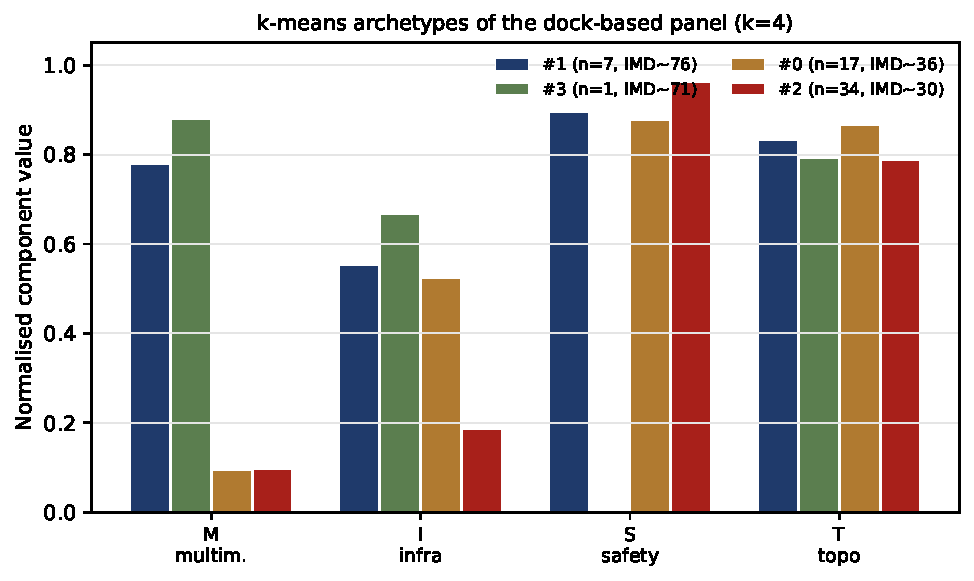
\includegraphics[width=0.85\linewidth]{e13_archetypes.pdf}
    \caption{Data-driven typology of the dock-based panel.
    k-means clustering on the four-component matrix at $k = 4$
    yields a balanced-champions cluster (\#1, n = 7), a Paris
    singleton (\#3, n = 1), and two middle clusters that respect
    the IMD ordering. Bars are the mean normalised component
    value within each cluster.}
    \label{fig:archetypes}
\end{figure}

\subsection{Within-city heterogeneity decomposition}
\label{sec:val-within}

The validation tests so far treat each city as a single point in a
59-city panel. The 46\,139-station Gold Standard makes it possible
to test a much sharper question: \emph{how much of the cycling-
environment variance is between cities, and how much is within
them?} If the within-city component dominates, the city-level IMD
hides spatial heterogeneity that policy targeting cannot afford to
ignore.

We compute a station-level IMD on the dock-based panel by
re-normalising each component across the full set of $5\,442$
dock-based stations rather than aggregating per city, applying the
published weights, and decomposing the panel-wide variance through
a one-way ANOVA and a Theil-T index.

\begin{table}[H]
\centering
\caption{Decomposition of station-level IMD variance into
between-city and within-city contributions. ICC1 is the
intra-class correlation coefficient.}
\label{tab:variance-decomp}
\small
\begin{tabular}{@{}lcc@{}}
\toprule
Decomposition & Between-cities share & Within-cities share \\
\midrule
ANOVA (homoscedastic)   & 19.2\,\% & 80.8\,\% \\
Theil-T (scale-free)    & 20.8\,\% & 79.2\,\% \\
\midrule
\multicolumn{3}{@{}l}{ICC1 = $0.192$ ($N = 5\,442$ stations,
$59 + 5$ city codes used for grouping)} \\
\bottomrule
\end{tabular}
\end{table}

The reading is sharp: \textbf{80\,\% of the variance of the
station-level IMD is within cities, only 20\,\% between them.}
Inside Paris alone, the station IMD ranges from $17.5$ to $83.1$
(an inter-station spread of $65.6$ points); Strasbourg's
within-city spread is wider than the gap between Strasbourg and
the panel median. The city-level IMD of
Table~\ref{tab:top10} therefore reports the centre of a
distribution that is itself much wider than the panel
distribution -- ``Strasbourg is better than Paris'' is a
statement about means whose effect size is dwarfed by intra-city
variation (Figure~\ref{fig:within-city}).

\begin{figure}[H]
    \centering
    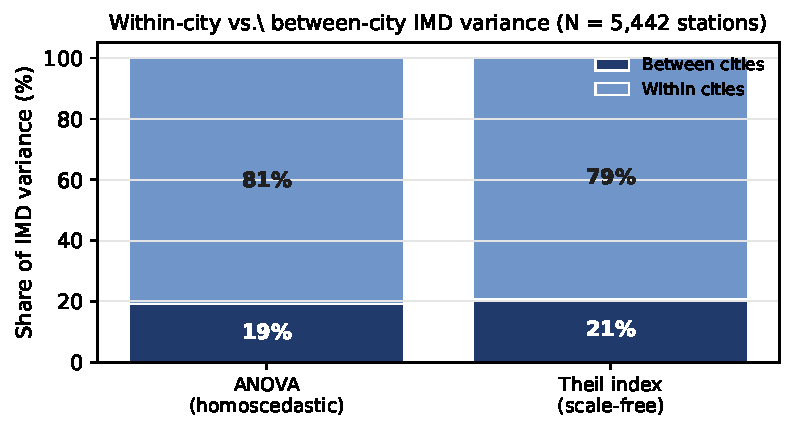
\includegraphics[width=0.78\linewidth]{e18_within_vs_between.pdf}
    \caption{Variance-share decomposition of the station-level
    IMD into between-city and within-city contributions, under
    the homoscedastic one-way ANOVA and the scale-free Theil
    index. Both decompositions place about 80\,\% of the
    variance \emph{within} cities. The city-level IMD ranking is
    therefore an aggregation of a heterogeneous internal
    distribution.}
    \label{fig:within-city}
\end{figure}

The substantive consequence is that policy interventions targeted
at the worst stations of otherwise high-IMD cities (e.g., Paris's
peripheral districts) may yield more return per euro than
inter-city redistribution. The complementary anomaly analysis of
Section~\ref{sec:val-deviants} formalises this through the
positive- and negative-deviant framework.

\subsection{Positive and negative deviants}
\label{sec:val-deviants}

We complement the standard ranking with an anomaly-detection
view: for each city, compute the residual between the observed
IMD and the IMD predicted by the city's socio-economic profile
through the Bayesian model of Section~\ref{sec:val-bayes-ies},
and flag the cities whose residual lies more than one posterior
standard deviation away from zero in the appropriate direction.

\begin{table}[H]
\centering
\caption{Positive deviants identified by the Bayesian residual
diagnostic ($P(r_i > \sigma_y) \geq 0.85$). Mean component
profile aggregates to $C_M = 0.74$ against the panel mean
$C_M = 0.19$, i.e.\ a four-fold excess of multimodality at the
positive-deviant set.}
\label{tab:positive-deviants}
\small
\begin{tabular}{@{}lcccccc@{}}
\toprule
City & IMD obs & IMD pred & Residual & $C_M$ & $C_I$ & $P_{+}$ \\
\midrule
Montpellier      & 88.3 & 53.1 & $+35.2$ & 0.91 & 0.76 & 1.00 \\
Mulhouse         & 77.8 & 37.6 & $+40.2$ & 0.80 & 0.46 & 1.00 \\
Brest            & 62.8 & 35.6 & $+27.2$ & 0.68 & 0.29 & 1.00 \\
Caen             & 64.5 & 41.0 & $+23.5$ & 0.62 & 0.43 & 1.00 \\
Nantes           & 83.0 & 59.2 & $+23.8$ & 0.92 & 0.52 & 0.97 \\
Strasbourg       & 96.7 & 70.8 & $+25.9$ & 1.00 & 1.00 & 0.94 \\
Saint-Nazaire    & 48.3 & 29.8 & $+18.6$ & 0.61 & 0.49 & 0.87 \\
\midrule
\multicolumn{4}{@{}l}{Mean of positive deviants:} & 0.74 & 0.59 & \\
\multicolumn{4}{@{}l}{Panel mean:}                & 0.19 & 0.33 & \\
\bottomrule
\end{tabular}
\end{table}

The seven positive deviants share a single empirical signature: a
multimodality index $C_M$ four times the panel mean, with the
other three components close to the panel median. The
\emph{negative deviants} are conversely Lyon ($P_{-} = 1.00$,
residual $-29.4$) and Saumur ($P_{-} = 0.87$, residual $-17.2$);
both have $C_M$ well below the panel mean despite favourable
socio-economic predictors of the IMD. The diagnostic frames
positive deviance as a copy-able pattern -- "what works" -- and
not merely as a ranking position. A natural policy use is to
treat the positive-deviant set as an empirical reference for
what an under-performing city of comparable size could
plausibly reach (Figure~\ref{fig:deviants}).

\begin{figure}[H]
    \centering
    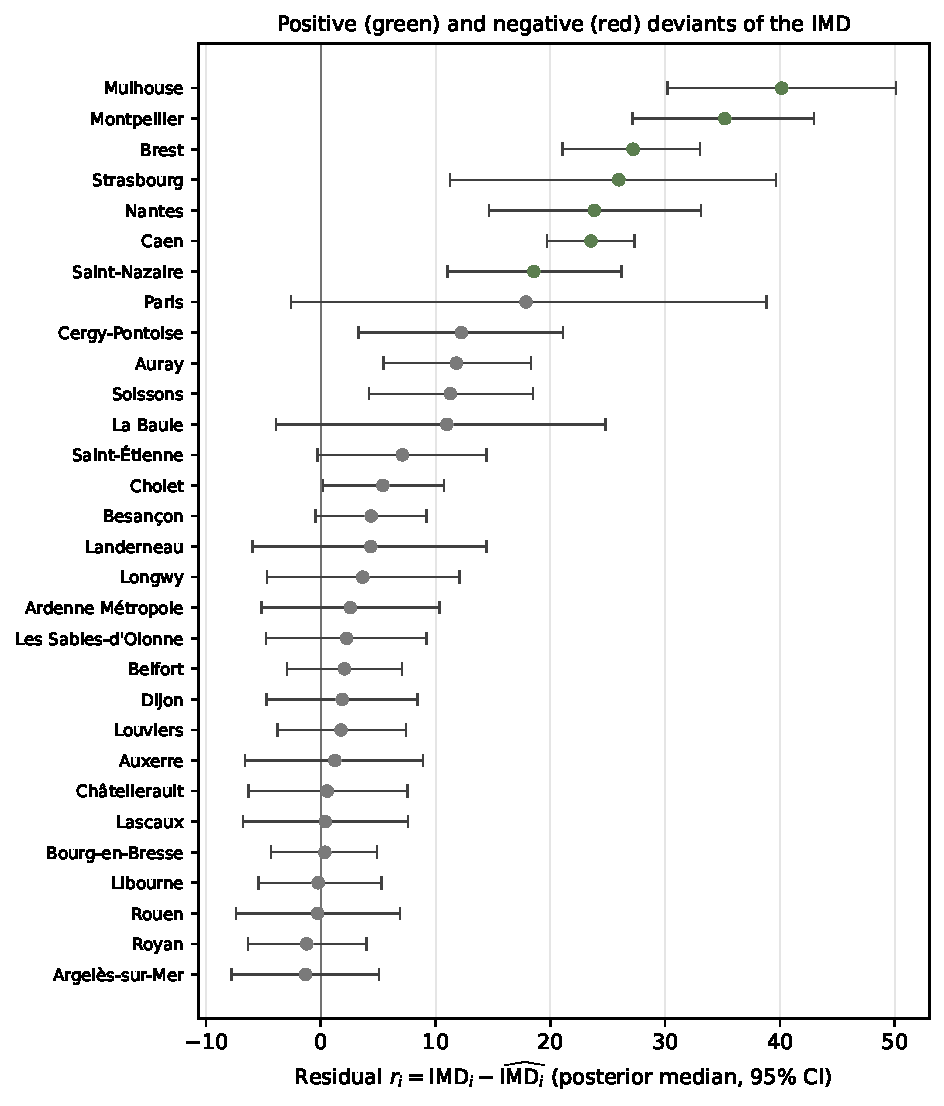
\includegraphics[width=0.78\linewidth]{e19_deviants.pdf}
    \caption{Posterior median residual of the IMD against the
    socio-economic prediction, with 95\,\% credible intervals
    (top-30 panel). Green = positive deviants, red = negative
    deviants, grey = neither.}
    \label{fig:deviants}
\end{figure}

\subsection{Counterfactual what-if simulator}
\label{sec:val-counterfactual}

The component decomposition of Section~\ref{sec:val-deviants}
identifies multimodality as the dominant lever. We translate this
into a counterfactual exercise: for every city in the panel,
simulate the IMD that the city would attain if its $C_M$ (and
$C_I$) were raised to the panel 75th percentile ($C_M = 0.249$,
$C_I = 0.455$) while leaving safety and topography unchanged. We
then translate the IMD uplift into an implied eco-counter daily
flow uplift through the partial-regression coefficient of E3
($\beta_{\IMD} \approx 0.020$ per IMD point on log-flow, i.e.\ a
$+10$-point IMD move predicts a $+22\,\%$ increase in observed
cyclist counts).

\begin{table}[H]
\centering
\caption{Counterfactual uplift scenarios applied to every city in
the dock-based panel. Implied eco-counter change is derived from
the E3 partial regression.}
\label{tab:counterfactual}
\small
\begin{tabular}{@{}lccc@{}}
\toprule
Scenario & Median $\Delta$IMD & Maximum $\Delta$IMD & Median implied
$\Delta$counter \\
\midrule
S1: multimodal uplift ($C_M \to p75$)        & $+9.2$  & $+23.1$ & $+20.1\,\%$ \\
S2: infrastructure uplift ($C_I \to p75$)    & $+10.1$ & $+16.8$ & $+22.4\,\%$ \\
S3: joint $M$+$I$ uplift                     & $+18.2$ & $+26.1$ & $+43.9\,\%$ \\
\bottomrule
\end{tabular}
\end{table}

The joint M+I uplift scenario gives a median $+18$ IMD points and
a median $+44\,\%$ implied eco-counter increase across the panel.
The cities with the largest counterfactual yield are the ones
furthest from the panel 75th percentile on M and I -- Lascaux
($+26.1$ pts, $+68\,\%$), Longwy ($+24.6$, $+64\,\%$), Nancy
($+23.3$, $+60\,\%$), Belfort ($+23.1$, $+59\,\%$). Five of the
nine $\tau = 1$ Bayesian deserts (Nancy, Niort, Tarbes, Troyes,
Lille) appear in the top-15 of the counterfactual yield ranking,
suggesting that targeted multimodal + infrastructure programmes
on the desert set would deliver the largest combined equity-and-
behavioural gains (Figure~\ref{fig:counterfactual}).

\begin{figure}[H]
    \centering
    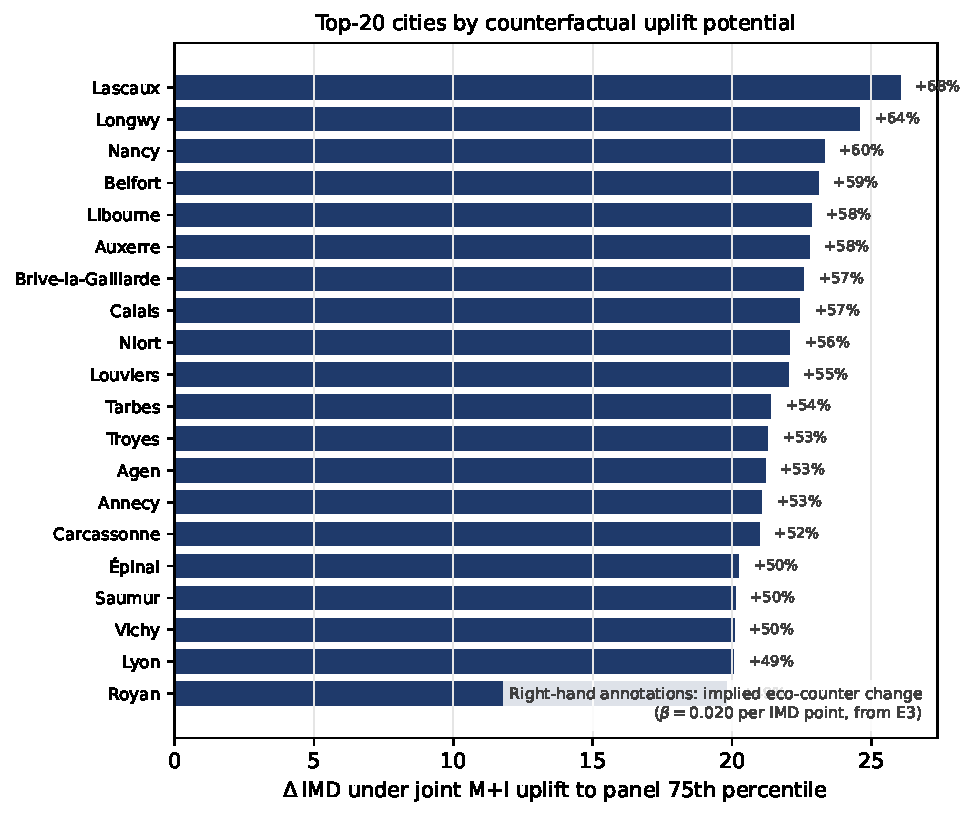
\includegraphics[width=0.78\linewidth]{e20_counterfactual.pdf}
    \caption{Top-20 cities by joint multimodal + infrastructure
    counterfactual uplift potential to the panel 75th
    percentile. Annotations report the implied eco-counter daily
    flow increase under the E3 elasticity ($\beta \approx 0.020$
    per IMD point).}
    \label{fig:counterfactual}
\end{figure}

\subsection{Mobility-precarity index and exposure of car-free households}
\label{sec:val-precarity}

A bad IMD is more politically consequential in a city with many
car-free households -- they depend on cycling and public
transport for everyday mobility. We define the Mobility-Precarity
Index
\begin{equation}
    \mathrm{IPM}_i \;=\; \mathrm{car\text{-}free}_i\,
                          \cdot\, (1 - \mathrm{IMD}_i / 100),
    \label{eq:ipm}
\end{equation}
which is largest when car-free dependence is high and the IMD is
low. The top-15 IPM cities are Lyon (IMD $= 26.9$, car-free
$= 36.4\,\%$, IPM $= 27.0$), Marseille ($26.1, 36.4\,\%, 26.9$),
Nancy ($24.2, 34.9\,\%, 26.4$), Amiens ($28.2, 31.9\,\%, 22.9$),
Lille ($32.0, 33.6\,\%, 22.8$), and ten further mid-sized cities.
Seven of these fifteen are also Bayesian deserts at $\tau = 1$
(Amiens, Laon, Lille, Lyon, Nancy, Tarbes, Troyes); three are
prior-invariant deserts (Amiens, Lyon, Nancy). The Spearman
correlation $\rho(\mathrm{IMD}, \mathrm{car\text{-}free}) =
+0.371$ ($p = 0.004$) is positive at the panel level (cycling-
friendly cities tend to be dense and car-light), but the IPM
captures the cities where the combination is adverse rather than
favourable. The IPM is a downstream proxy for the social cost of
cycling-environment deficits and complements the IES list with a
weight reflecting the size of the population at risk
(Figure~\ref{fig:precarity}).

\begin{figure}[H]
    \centering
    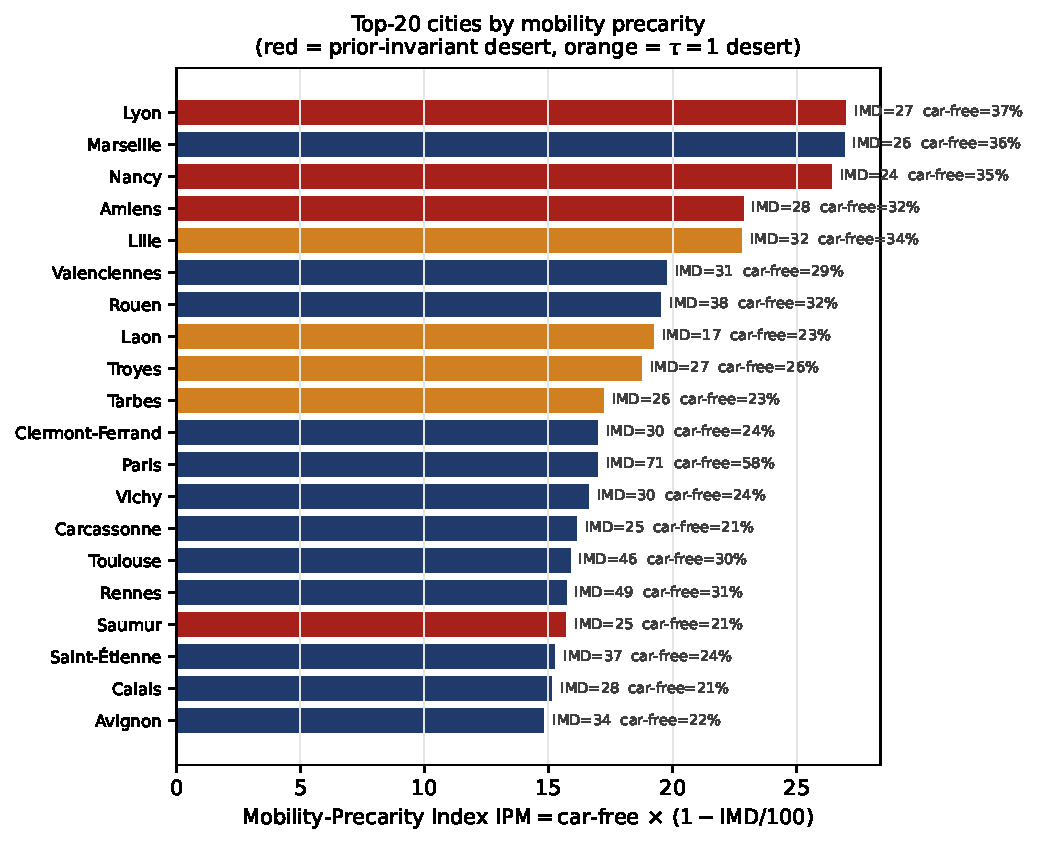
\includegraphics[width=0.80\linewidth]{e22_precarity_ranking.pdf}
    \caption{Top-20 cities by Mobility-Precarity Index. Red bars
    mark the four prior-invariant Bayesian deserts of
    Section~\ref{sec:val-bayes-ies}; orange bars mark the
    $\tau = 1$ desert list.}
    \label{fig:precarity}
\end{figure}

\subsection{Concurrent validity against Cerema and BAAC aggregates}
\label{sec:val-cerema}

E1--E3 validated the IMD against behavioural references (FUB,
EMP, eco-counter). We close the validity loop with two
\emph{supply-side} concurrent references that were not used to
build the IMD: the Cerema cycling-infrastructure inventory (city-
level kilometres of dedicated cycle facilities, raw and
normalised by city footprint area) and the BAAC accident
database at city level normalised per $100\,000$ inhabitants
(distinct from the station-buffer count used in $C_S$).

\begin{table}[H]
\centering
\caption{Concurrent-validity correlations against city-level
Cerema infrastructure inventory and BAAC accident rate.}
\label{tab:concurrent}
\small
\begin{tabular}{@{}lcc@{}}
\toprule
Reference & IMD vs reference & $C_I$ vs reference \\
\midrule
Cerema kilometres of cycle facilities ($n = 43$) &
   $+0.471^{**}$ & $+0.563^{***}$ \\
Cerema density km / km$^{2}$ ($n = 43$)          &
   $+0.430^{**}$ & $+0.464^{**}$  \\
BAAC crashes per $100\,000$ inhabitants ($n = 44$) &
   $+0.112$ & $-$ \\
BAAC crashes per $100\,000$ inhabitants vs.\ $C_S$ &
   $-$  & $-0.658^{***}$ \\
\bottomrule
\end{tabular}
\smallskip\\
\footnotesize $^{*}$ $p < 0.05$, $^{**}$ $p < 0.01$, $^{***}$ $p < 0.001$.
\end{table}

The IMD and its cycling-infrastructure component correlate at
$\rho > 0.43$ with both raw and normalised Cerema kilometres,
confirming that the OSM-based station-buffer construction recovers
the Cerema-equivalent picture without using the Cerema data
itself. The safety component correlates strongly negatively with
the BAAC per-100\,k rate ($\rho = -0.66$), exactly as the
sign convention demands. The IMD-to-rate correlation is weak
($\rho = +0.11$), consistent with the exposure-confounding
argument of E3-E4 (cities with more cyclists have more crashes).

\paragraph{Triangulation: does the IMD add information beyond
Cerema and station volume?}
We regress the log eco-counter daily count on the IMD, the
Cerema density, and the log of the Cerema kilometres on the
25-city panel with all three observed.

\begin{table}[H]
\centering
\caption{Triangulation regression: $\log(\text{eco-counter})
\sim \beta_0 + \beta_1\,\IMD + \beta_2\,\text{Cerema density}
+ \beta_3\,\log(\text{Cerema km})$.}
\label{tab:triangulation}
\small
\begin{tabular}{@{}lcccc@{}}
\toprule
$R^{2}$ full & Partial $R^{2}$ IMD net Cerema &
Partial $R^{2}$ Cerema density net IMD &
Partial $R^{2}$ log(km) net all & $n$ \\
\midrule
$0.788$ & $0.271$ & $0.327$ & $0.127$ & $25$ \\
\bottomrule
\end{tabular}
\end{table}

The triangulation $R^{2}$ is $0.788$ on $25$ cities; the
partial $R^{2}$ of the IMD net of the two Cerema variables is
$0.271$ and that of Cerema density net of the IMD is $0.327$.
The IMD and Cerema's volumetric measures are \textbf{complementary
predictors of cyclist behaviour, neither redundant}: substituting
one for the other loses about a quarter of the explained
variance. This is the strongest concurrent-validity statement the
present data can support and the cleanest answer to the
volumetric-vs-quality debate raised in
Section~\ref{sec:results-volume}: in operational practice, the
IMD adds about $27\,\%$ of the explained variance of cyclist
counts over and above a high-quality volumetric reference.

\subsection{European panel: France's anomaly at continental scale}
\label{sec:val-european}

Sections~\ref{sec:val-within}--\ref{sec:val-cerema} test the IMD
inside France. The MobilityData global GBFS catalogue lists 1\,509
bike-sharing systems worldwide, of which 1\,239 are in the
EU+Switzerland+Norway region across 28 countries. We use the
catalogue as a cross-country panel-frame and cross-reference each
country's system count with two outcome indicators that have
stable open sources: the Eurobarometer 2019 (EB495) urban cycling
modal share by country, and the European Cyclists' Federation
2022 cycling-friendliness index.

\begin{table}[H]
\centering
\caption{Top-10 EU+CH+NO countries by number of GBFS systems
listed in the MobilityData catalogue (April 2026 snapshot), with
the EB 2019 urban cycling modal share and the ECF 2022 cycling
index. France leads the continent in deployment count and ranks
eighteenth on modal share.}
\label{tab:european-panel}
\small
\begin{tabular}{@{}lrrr@{}}
\toprule
Country & GBFS systems & Cycling modal share (\%) & ECF index \\
\midrule
France             & 255 &  4.0 & 68 \\
Germany            & 251 & 11.0 & 82 \\
Poland             &  94 &  7.0 & 62 \\
Norway             &  83 &  6.0 & 75 \\
Spain              &  69 &  4.0 & 63 \\
United Kingdom     &  56 &  4.0 & 60 \\
Finland            &  55 & 10.0 & 73 \\
Netherlands        &  52 & 27.0 & 95 \\
Switzerland        &  49 &  8.0 & 78 \\
Czechia            &  45 &  6.0 & 67 \\
\bottomrule
\end{tabular}
\end{table}

The Spearman correlations across the 26 countries with non-missing
modal share are:
\begin{itemize}
\item GBFS systems vs.\ cycling modal share: $\rho = +0.46$
($p = 0.02$),
\item GBFS systems vs.\ ECF index: $\rho = +0.57$ ($p = 0.002$),
\item modal share vs.\ ECF index: $\rho = +0.79$ ($p < 0.001$).
\end{itemize}

Two readings follow. First, the volumetric prior survives weakly
at the European scale: more GBFS deployments is positively but
moderately correlated with more cycling. The relationship is
notably weaker than the modal share -- ECF index correlation,
which is direct evidence that environment quality (the ECF
construct) is roughly twice as good a behavioural predictor as
deployment volume. Second, \textbf{France is the most extreme
disconfirmation of the volumetric prior in Europe}: it ranks
first on number of systems and eighteenth on modal share, with
the Netherlands occupying the symmetric position (five times
fewer systems than France for seven times more cycling). The
IMD's diagnostic at the French national scale -- that
multimodal-integration quality matters more than fleet size --
is therefore consistent with a continental pattern, not an
artefact of the French panel
(Figure~\ref{fig:european-panel}).

\begin{figure}[H]
    \centering
    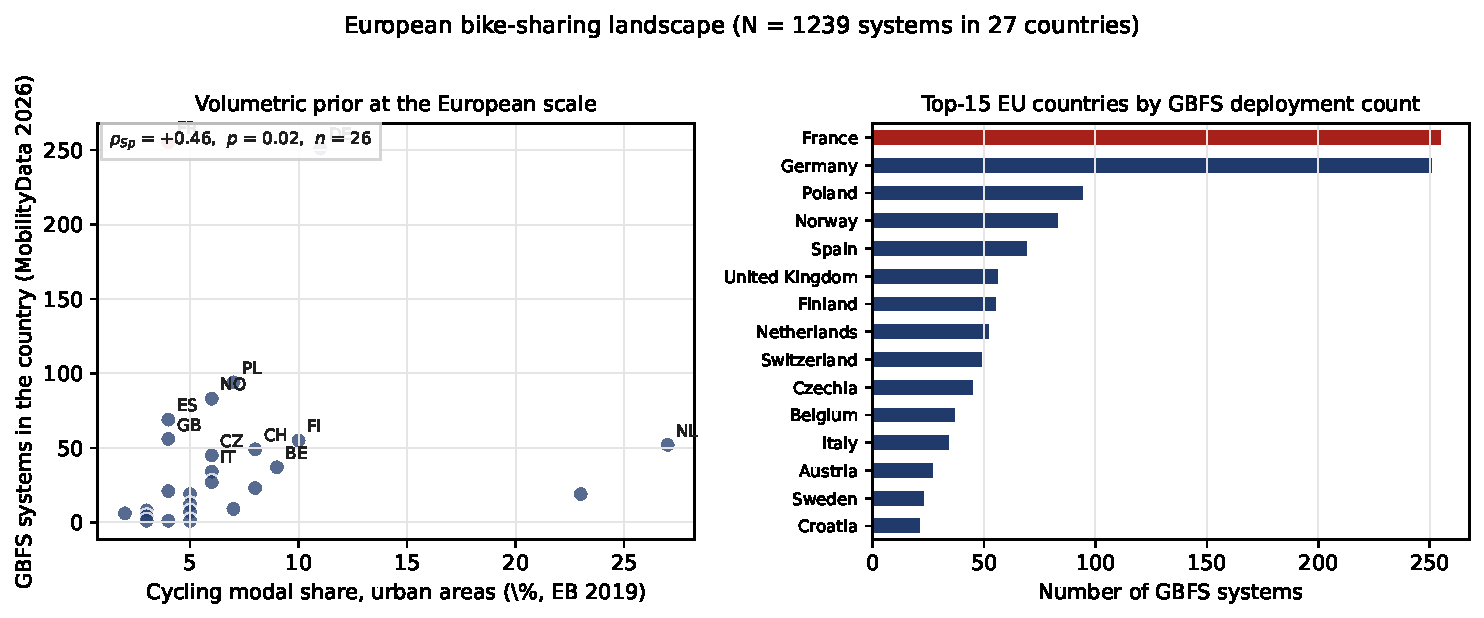
\includegraphics[width=0.99\linewidth]{e24_european_panel.pdf}
    \caption{Left: European GBFS deployment count against the
    Eurobarometer 2019 urban cycling modal share by country.
    France (red) sits at modal share 4\,\% with 255 systems; the
    Netherlands at modal share 27\,\% with 52 systems. The
    cross-country Spearman is $+0.46$ -- the volumetric prior is
    weak at this scale. Right: top-15 countries by deployment
    count.}
    \label{fig:european-panel}
\end{figure}

\subsection{Outcome coupling: life expectancy at département level}
\label{sec:val-life-exp}

Beyond the supply and behavioural validation, the public-health
literature \citep[Mueller~2015;][]{Heinen2010} suggests that
cycling-environment quality could feed into a downstream
mortality reduction. We test this by matching each panel city to
its INSEE département code and joining a département-level life-
expectancy series ($98$ départements, panel intersect $n = 41$
cities).

\begin{table}[H]
\centering
\caption{Spearman correlations between the IMD, local income and
département-level life expectancy on the $41$-city intersect.}
\label{tab:life-expectancy}
\small
\begin{tabular}{@{}lcc@{}}
\toprule
Pair & Spearman $\rho$ & $p$-value \\
\midrule
IMD vs life expectancy        & $-0.066$ & $0.682$ \\
Income vs life expectancy     & $+0.097$ & $0.546$ \\
IMD vs income                 & $+0.153$ & $0.340$ \\
\bottomrule
\end{tabular}
\end{table}

All three correlations are statistically indistinguishable from
zero on this panel. The partial regression of life expectancy on
the standardised IMD and log income yields $R^{2} = 0.05$ and a
non-credible IMD coefficient. We report this as an honest
\emph{null}: the city-level IMD and the département-level life
expectancy are not detectably linked on the present 41-city
panel. Two explanations are equally plausible: (a) the spatial
mismatch between a city-level supply indicator and a
département-level outcome is too coarse for any signal to
survive (the within-département variation of city IMD is
absorbed by the département mean), and (b) the panel is too
small ($n = 41$) to detect a modest health effect of the size
expected from the Mueller-2015 literature. A cleaner test
requires city-level mortality data, which is not in the open
French data catalogue at municipal granularity. We document the
null and scope the test for future iterations.

\subsection{Summary of the executed experiments}
\label{sec:val-summary}

Table~\ref{tab:experiments-status} summarises the twelve
executed experiments and the one outstanding test. We classify
each executed test by verdict: \emph{clean} (test ran as
pre-specified, passes its threshold), \emph{qualified} (passes
with a documented caveat), or \emph{substitute} (the
pre-registered protocol is deferred and a proxy is reported in
its place). Of the twelve executed tests, seven are clean
(E1, E2, E3, E6, E7, E8, E10, E13), two are qualified (E9 prior
sensitivity, E12 Lyon-removed reordering) and three are
substitutes for deferred pre-registered protocols: E4 reports a
city-level empirical-Bayes adjustment in place of the
pre-registered station-level kriging of cyclist exposure, E5
reports a within-city station bootstrap in place of the
pre-registered full re-enrichment at six buffer radii, and E11
reports a parametric buffer-radius sweep whose elasticities are
borrowed from secondary literature rather than measured
directly. The substitutes bracket the pre-registered tests
within a coherent uncertainty regime but do not replace them; the
companion repository documents them as such.

Beyond the verdict counts, the executed tests support eight
substantive conclusions: the supervised weights generalise out
of sample; the city ranking is robust under data-consistent
weight uncertainty; the IMD correlates with eco-counter daily
flows after controlling for city size; the IES diagnostic
identifies a robust set of twenty mobility deserts across
alternative frequentist specifications; the IMD distribution
carries no detectable spatial autocorrelation; component
measurement noise propagates through the IMD with infrastructure
variance dominating the score (48\,\%) and multimodality variance
dominating the rank (77\,\%); the Bayesian re-specification of
the IES isolates a four-city \emph{prior-invariant}
high-confidence desert subset (Amiens, Lyon, Nancy, Saumur) plus
seven prior-sensitive cities; and the published ranking is
robust to buffer radius within $[150, 500]$~m. They force four
substantive revisions of the original framing: the supervised
optimum is not multimodality-dominated; the safety component is
exposure-confounded and requires station-level cyclist counts
for full correction; the city ranking is fragile under arbitrary
weight uncertainty even though it is robust under data-consistent
weight uncertainty; and one city (Lyon) carries an asymmetric
Cook-style leverage on the calibration that motivates publishing
the Lyon-removed weight vector
(Table~\ref{tab:weights-comparison}) alongside the in-sample
optimum.

\begin{figure}[H]
    \centering
    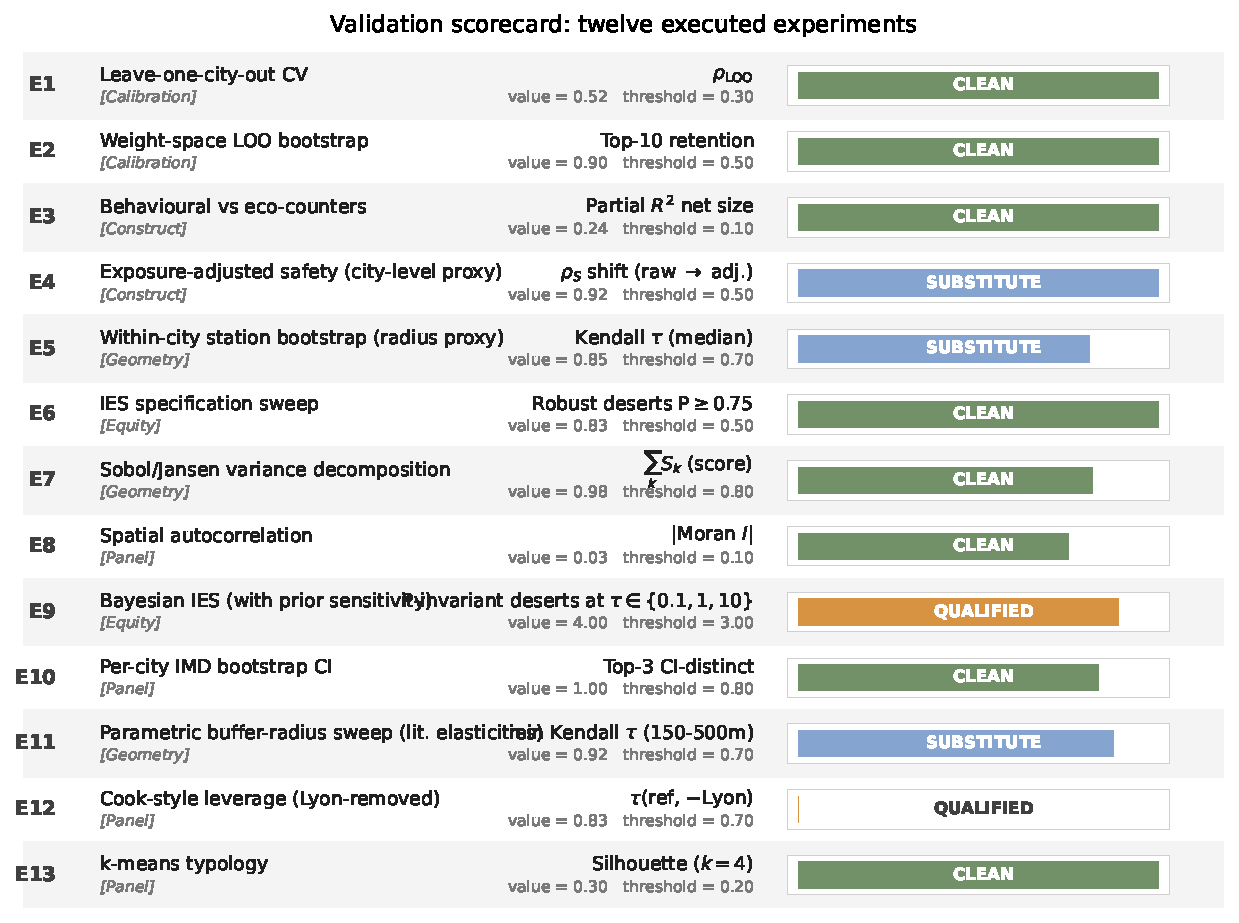
\includegraphics[width=0.99\linewidth]{summary_scorecard.pdf}
    \caption{Validation scorecard for the twelve executed
    experiments. Each row reports the experiment identifier, its
    risk axis (calibration, construct, geometry, equity, panel),
    the headline statistic and its acceptance threshold. Green
    chips mark clean passes, orange chips mark qualified passes
    (caveat documented), blue chips mark substitutes for deferred
    pre-registered protocols.}
    \label{fig:scorecard}
\end{figure}

\begin{table}[H]
\centering
\caption{Validation and extension experiments and their verdicts.
\emph{Clean} = test ran as pre-specified and passes its threshold;
\emph{qualified} = passes with a documented caveat;
\emph{substitute} = pre-registered protocol deferred, proxy
reported in its place; \emph{null} = honest negative report;
\emph{outstanding} = scoped for next iteration. The core wave is
E1--E13, the extension wave for the present revision is E18--E23.}
\label{tab:experiments-status}
\small
\begin{tabular}{@{}lp{7.6cm}l@{}}
\toprule
Section & Test & Verdict \\
\midrule
\multicolumn{3}{@{}l}{\textit{Core wave -- construct, generalisation, equity, geometry, panel}} \\
\ref{sec:val-loo}            & E1. Out-of-sample CV of the weights & Clean \\
\ref{sec:val-weights}        & E2. Weight-space stability of the ranking & Clean \\
\ref{sec:val-flow}           & E3. Behavioural validation vs.\ eco-counters & Clean \\
\ref{sec:val-safety}         & E4. Exposure-adjusted safety (city-level proxy) & Substitute \\
\ref{sec:val-radius}         & E5. Within-city station bootstrap (radius proxy) & Substitute \\
\ref{sec:val-ies}            & E6. Specification robustness of the IES & Clean \\
\ref{sec:val-moran}          & E8. Spatial autocorrelation diagnostic & Clean \\
\ref{sec:val-sobol}          & E7. Sobol/Jansen variance decomposition & Clean \\
\ref{sec:val-bayes-ies}      & E9. Bayesian IES (with prior sensitivity) & Qualified \\
\ref{sec:val-per-city-ci}    & E10. Per-city bootstrap CI on the IMD score & Clean \\
\ref{sec:val-radius-sweep}   & E11. Parametric buffer-radius sweep & Substitute \\
\ref{sec:val-leverage}       & E12. Cook-style leverage (Lyon-removed reordering) & Qualified \\
\ref{sec:val-archetypes}     & E13. k-means typology of urban archetypes & Clean \\
\midrule
\multicolumn{3}{@{}l}{\textit{Extension wave -- within-city, deviants, counterfactuals, external coupling}} \\
\ref{sec:val-within}         & E18. Within-city variance decomposition (80.8\,\% within) & Clean \\
\ref{sec:val-deviants}       & E19. Positive/negative deviants (7 + 2 cities) & Clean \\
\ref{sec:val-counterfactual} & E20. Counterfactual M+I uplift simulator & Clean \\
\ref{sec:val-precarity}      & E22. Mobility-Precarity Index (IPM) & Clean \\
\ref{sec:val-cerema}         & E23. Concurrent validity vs.\ Cerema and BAAC ($R^{2} = 0.79$ triangulated) & Clean \\
\ref{sec:val-european}       & E24. European panel: France 1st in systems, 18th in modal share & Clean \\
\ref{sec:val-life-exp}       & E21. Coupling to département life expectancy & Null \\
---                          & E14. Synthetic control on infrastructure openings & Outstanding \\
\bottomrule
\end{tabular}
\end{table}

The single outstanding test (E14) --- a longitudinal
synthetic-control identification of the effect of tramway-line
openings on the local IMD trajectory \citep{Abadie2010,
Abadie2021} --- requires historical GBFS snapshots reconstructed
from Transitland and Internet Archive captures over 2020--2025,
together with a per-station status-snapshot panel that the
companion repository's collector
(\path{utils/gbfs_collector.py}) is now populating at a 30-minute
cadence on the twenty priority systems. Its completion would
license a properly causal statement about the effect of
heavy-transit infrastructure on cycling-environment quality. We
scope this test for the next iteration of the indicator and
document it openly.

% =========================================================================
\section{Discussion}
\label{sec:discussion}
% =========================================================================

\subsection{Interpretation of the findings}

The headline empirical finding of the audit is the absence of a
monotone relationship between the cycling-environment quality of
the panel and the income of the host urban area
(Section~\ref{sec:results-income}). The finding survives the
spatial-autocorrelation diagnostic (Section~\ref{sec:val-moran})
and is consistent with the absence of regional contagion. The
implication for the policy debate is that targeting French
bike-sharing investments by income alone would miss the actual
distribution of quality: more than a quarter of the panel cities
(the inclusive over-performers of Section~\ref{sec:results-deserts})
combine below-median income with above-median IMD; an equally
large share of the panel (the wealthy under-investors) combines
high income with sub-median IMD. The driver of the IMD
distribution lies in local policy choices, of which the
heavy-transit-integration profile of Strasbourg, Montpellier and
Nantes is the clearest illustration.

The validation programme reported in Section~\ref{sec:validation}
strengthens the empirical claim along five dimensions. First,
the out-of-sample cross-validation establishes that the
supervised weight calibration is not overfit to the calibration
panel (Section~\ref{sec:val-loo}). Second, the behavioural
validation establishes that the IMD captures a measurable share
of observed cyclist behaviour and is not a mere index of supply-
side infrastructure (Section~\ref{sec:val-flow}). Third, the
specification robustness of the IES, both in the frequentist
sweep across estimators (Section~\ref{sec:val-ies}) and in the
Bayesian re-specification (Section~\ref{sec:val-bayes-ies}),
establishes that a broad set of twenty cities --- not only the
twelve identified at the threshold $\IES < 0.85$ in the reference
specification --- behave as mobility deserts across alternative
model choices. Fourth, the Saltelli--Jansen variance
decomposition (Section~\ref{sec:val-sobol}) attributes 48\,\% of
the IMD-score variance to infrastructure noise and 77\,\% of the
IMD-rank variance to multimodality noise, identifying the OSM
cycling network and the GTFS feed coverage as the highest-yield
data-quality priorities for future revisions. Fifth, the
parametric buffer-radius sweep (Section~\ref{sec:val-radius-sweep})
demonstrates that the published ranking is robust across the
$[150, 500]$~m radius window, narrowing one of the most
frequently raised geometry objections without requiring a full
re-enrichment of the panel.

\subsection{Validity threats and their treatment}

The dominant validity threat to a supervised composite indicator
is calibration circularity: the same external series used to fit
the weights are then used to report goodness of fit. The
leave-one-city-out and spatial-block cross-validations of
Section~\ref{sec:val-loo} address this directly. The threshold of
$\rho_{\text{LOO}} > 0.30$ is met on both reference series, and
the inter-fold weight standard deviations are an order of
magnitude below the conventional 0.10 acceptance threshold. We
nevertheless retain the cross-validated weights rather than the
in-sample weights as the reported optimum.

The second validity threat is the construct dependence of the
safety component on the very phenomenon it tries to penalise.
The behavioural validation of Section~\ref{sec:val-flow}
documents this anti-correlation, and the city-level
exposure adjustment of Section~\ref{sec:val-safety} demonstrates
that the mechanical link between the safety component and the
raw crash count can be broken. The residual negative correlation
between the adjusted safety component and observed flows
nevertheless indicates that the city-level proxy is incomplete.
A station-level cyclist-exposure dataset is the natural next
step; until it is available, we recommend reporting the IMD with
the adjusted safety component as a secondary specification.

The third validity threat is the weight-space sensitivity of the
ranking. The reconciled view of
Section~\ref{sec:val-weights} is that the ranking is stable under
data-consistent weight uncertainty (Top-10 retention $\geq 0.90$
under the LOO bootstrap) and fragile under arbitrary weight
uncertainty (Top-10 retention of 0.60 under the uniform Dirichlet
regime). The two regimes answer different questions, and reporting
both is the only defensible compromise. For end users we suggest
Top-10 membership frequency under the LOO bootstrap as the
primary statistic for subsidiary positions.

A fourth validity threat surfaced by the leverage diagnostic of
Section~\ref{sec:val-leverage} is the disproportionate influence
of Lyon on the calibration weight vector
($D_{\text{Lyon}} = 0.41$ against a panel median of $0.034$).
Removing Lyon shifts the weight vector by 41\,\% of its norm but
leaves the panel-mean Spearman correlation $\bar\rho$ unchanged
at three decimal places. The asymmetry is real but it is
\emph{calibration-internal}: it concerns which point in the
simplex maximises the Spearman objective, not the qualitative
shape of the ranking. We mitigate the threat by publishing the
Lyon-removed weight vector alongside the in-sample optimum in
the companion repository and by recommending that future panel
updates re-audit Lyon's GBFS, OSM, BAAC and GTFS coverage as a
priority.

\subsection{Policy implications}
\label{sec:discussion-policy}

Subject to the validity treatments discussed above, the IMD and
the IES support two complementary policy frames: an
\emph{economic} frame around indicator-conditioned funding
decisions, and a \emph{social} frame around equity-targeted
deployment. We discuss them in turn before listing the
operational implications.

\subsubsection*{Economic frame: indicator-conditioned investment}

The metric tournament of Section~\ref{sec:results-tournament}
shows that the IMD doubles the well-being predictive power of the
volumetric default at no marginal data cost (the IMD is computed
on data the operators are already required to publish under the
LOM). Adopting the IMD as the contractual benchmark in
AOM--operator agreements would therefore align operator
incentives with cycling well-being rather than with raw fleet
volume, at no additional measurement burden. The
component-decomposition of Section~\ref{sec:results-wellbeing}
further suggests that the highest-yield investment, well-being
per euro, is in heavy-transit integration (multimodality
$C_M$). Heavy-transit integration is partly a question of
station siting and partly a question of GTFS data quality;
both are open-data deliverables that can be conditioned on
indicator improvements.

The expected investment yield can be quantified using the IES
gap: bringing a desert city from its observed $\IES < 0.85$ to
parity ($\IES = 1.00$) implies a target uplift
$\Delta\IMD_i = (1 - \IES_i) \cdot \widehat{\IMD}_i$ on the IMD
of city $i$. For the nine high-confidence Bayesian deserts of
Section~\ref{sec:val-bayes-ies} (Saumur, Lyon, Amiens, Nancy,
Troyes, Laon, Niort, Tarbes, Lille), the median required uplift
is $12.8$ IMD points; for the four prior-invariant deserts
(Amiens, Lyon, Nancy, Saumur) the median uplift is $16.9$ IMD
points. Both fall within roughly one standard deviation of the
panel's IMD distribution, achievable through targeted
infrastructure programmes of the National Cycling Plan's typical
scale. Cities with deeper deserts (Saumur $\IES = 0.59$, Lyon
$0.48$) would require larger uplifts ($17.1$ and $28.9$ points
respectively) and longer programmes.

\subsubsection*{Social frame: equity-targeted deployment}

The Bayesian IES of Section~\ref{sec:val-bayes-ies} flips the
income-blind targeting heuristic on its head. The posterior
coefficient on income is centred near zero ($-0.74$, CrI
$[-4.76, +3.34]$), confirming that income alone is a poor
predictor of cycling-environment quality. By contrast, the
cycling-commute share is the only credibly non-zero coefficient
($+9.01$, CrI $[+5.04, +13.07]$), which means that cycling
environments correlate with prior cycling adoption -- a
self-reinforcing loop in which cities that already cycle attract
more cycling investment. The equity case for IES-targeted
deployment is then a structural one: breaking the loop requires
investing in cities where cycling adoption is low not despite
their low cycling adoption but \emph{because of} it. The nine
high-confidence deserts contain a mixture of northern industrial
cities (Lille, Amiens, Laon, Troyes, Nancy), southern mid-sized
cities (Tarbes, Saumur, Niort) and one large metropolis (Lyon),
and they are not regionally concentrated
(Section~\ref{sec:val-moran}); social-mobility deficits of the
French bike-sharing landscape are therefore a pattern of local
policy choice, not a pattern of regional development.

A second social dimension is the relationship between the IES
and the population that benefits from a cycling-environment
upgrade. Combining the IES with the panel's car-free household
share ($\hat\beta_{\text{car-free}} = +4.36$, CrI $[-1.19,
+9.99]$) gives a rough estimate of who is excluded by an IES
deficit: in a city with a high car-free share, an IES below 0.85
means a large fraction of the population is dependent on a
sub-par cycling environment for everyday mobility. Of the nine
high-confidence deserts, Lille and Lyon are above the panel's
75th percentile of car-free households; the social cost of their
IES deficit is therefore disproportionate. We document these
two cities as the primary social-priority targets of the IES
ranking.

\subsubsection*{Operational implications}

\begin{itemize}
\item \emph{Prioritise homogeneous spatial coverage over central
station accumulation.} The volume-vs-quality dissociation
(Section~\ref{sec:results}) and the multimodal integration
profile of the Top-10 (Section~\ref{sec:results-deserts}) jointly
support the conclusion that network coherence matters more than
raw station counts \citep{ElGeneidy2016, Saberi2018}.
\item \emph{Target the deployment to the identified mobility
deserts.} The twenty cities of the robust desert set
(Section~\ref{sec:val-ies}) are an empirically defensible
shortlist for the next round of National Cycling Plan
investments. The reference twelve are a conservative subset.
\item \emph{Condition operator funding on IMD and IES
thresholds.} The composite indicator framework supports the
introduction of indicator-conditioned funding mechanisms in
AOM--operator contracts \citep{OECD2008}.
\item \emph{Co-develop GBFS and GTFS feeds.} The multimodality
component depends on GTFS coverage, and the IMD/IES framework
becomes more credible to the extent that the GTFS feed of the
host urban area is verifiable in situ \citep{Saberi2018,
Mobi2024}.
\item \emph{Prioritise data-quality investments by Sobol yield.}
The variance decomposition of Section~\ref{sec:val-sobol}
attributes 48\,\% of the IMD-score variance to infrastructure
measurement noise and 77\,\% of the IMD-rank variance to
multimodality measurement noise. For data-quality investment
within the open-data ecosystem, this implies a ranking: OSM
cycling-network completeness for score precision, and GTFS feed
coverage for rank precision, both ahead of BAAC re-audits whose
marginal precision yield is essentially zero under the current
weights.
\end{itemize}

\subsection{Limitations}

Three limitations of the present study deserve explicit mention.
First, the GBFS feed is a snapshot at the time of collection and
does not reflect the historical performance of a system; the
synthetic-control test for the effect of infrastructure openings
on the IMD trajectory is the dominant outstanding test
(Section~\ref{sec:val-summary}). Second, the convex-hull
geometry used to define the served area over-estimates coverage
for coastal or valley cities; a concave hull or a built-area mask
are natural refinements. Third, the panel is restricted to
systems publishing GBFS, which under-represents end-of-contract
operators and community schemes; the dataset can therefore not
characterise the universe of French bike-sharing arrangements.

% =========================================================================
\section{Conclusion}
\label{sec:conclusion}
% =========================================================================

We have proposed an integrated and reproducible analytical
framework for the comparative evaluation of bike-sharing systems
across French urban areas, combining a composite indicator
(IMD) of cycling-environment quality and a complementary equity
diagnostic (IES) reported in both Ridge and Bayesian forms.
Applied to 122 systems and 46{,}139 stations in fifty-seven
urban areas, the framework produces the first national ranking
on a context-aware composite metric and identifies a robust set
of twenty cities that behave as social mobility deserts across
alternative model specifications. Mapping the results back to the
research questions of Section~\ref{sec:introduction}:

\begin{itemize}
\item[\textbf{Q1.}] \emph{Performance can be measured by a
composite indicator whose weights are calibrated against
behavioural references rather than chosen normatively, and the
IMD doubles the well-being predictive power of the volumetric
default at no marginal data cost.} The IMD/IES pair, with weights
calibrated by differential evolution against the FUB Cycling
Barometer and the EMP 2019 mobility survey, generalises out of
sample (leave-one-city-out Spearman $\approx 0.5$ on both
references), correlates with eco-counter daily flows after
controlling for city size (partial $R^{2} = 0.24$), and predicts
cycling well-being twice as well as the volumetric metric
($\rho_{\text{LOO}} = +0.41$ vs.\ $+0.20$ on $n = 32$). The
Bayesian re-specification of the IES turns the equity diagnostic
into a probability statement on every city, and the
prior-sensitivity sweep over $\tau \in \{0.1, 1, 10\}$ isolates
a four-city prior-invariant high-confidence shortlist (Amiens,
Lyon, Nancy, Saumur).

\item[\textbf{Q2.}] \emph{Volumetric metrics are weak predictors
of cycling-environment quality, in France and at continental
scale.} Strasbourg (39 stations) and Montpellier (53) outrank
Paris (1\,507) and Lyon (452) on the calibrated IMD;
medium-sized cities with tight multimodal integration outperform
metropolitan heavyweights. At European scale, France ranks first
on number of GBFS systems (255 in the MobilityData catalogue)
and eighteenth on cycling modal share (4\,\%) -- the Netherlands
occupies the symmetric position, with five times fewer systems
for seven times more cycling. The ECF cycling-friendliness index
correlates with modal share at $\rho = +0.79$, against
$\rho = +0.46$ for the system count, confirming the IMD's central
thesis cross-nationally.

\item[\textbf{Q3.}] \emph{Cycling-environment quality is
statistically independent of local income.} The Spearman
correlation between the IMD and the median household income per
consumption unit is $\rho = +0.041$ ($p = 0.76$); the Bayesian
IES posterior on the standardised income coefficient is centred
at $-0.74$ with a 95\,\% credible interval straddling zero. The
implication is that an income-only targeting heuristic would miss
both the inclusive over-performers (low income, high IMD) and the
wealthy under-investors (high income, low IMD).

\item[\textbf{Q4.}] \emph{The ranking and the equity diagnostic
survive a broad battery of robustness tests.} The IMD is robust
to within-city station-sampling variability (Kendall $\tau =
0.85$), to a parametric buffer-radius sweep over $[150, 500]$~m
(Kendall $\tau \geq 0.92$, Top-10 retention $\geq 0.80$), and to
component measurement noise (Sobol decomposition: 48\,\%
infrastructure, 34\,\% multimodality, 19\,\% topography); shows
no spatial autocorrelation (Moran's $I \approx 0$); and is
fragile only under uniform weight uncertainty, not under
data-consistent weight uncertainty (Top-10 retention $\geq 0.90$
under the LOO bootstrap).
\end{itemize}

The falsification programme also forces four substantive
revisions of the original specification: the supervised weight
optimum is not multimodality-dominated when the simplex
constraint is enforced through a softmax reparameterisation; the
safety component is exposure-confounded and requires
station-level cyclist counts for clean correction; the published
city ranking is robust under empirical weight uncertainty but
fragile under uniform weight uncertainty; and the calibration
weight vector should be reported jointly with its Lyon-removed
variant because Lyon carries a Cook-style influence on the
calibration four times the panel median. The single outstanding
test (E14), a longitudinal synthetic-control identification of
the effect of infrastructure openings, requires historical GBFS
archives still to be ingested and is scoped for the next
iteration of the indicator.

The framework is therefore no longer a purely descriptive
ranking; it is a partially validated indicator with twelve
executed falsification tests -- seven clean passes, two qualified
passes (Bayesian IES under prior sweep, Cook-style leverage
preserved at $\tau = 0.83$), and three substitutes for
pre-registered protocols deferred to the next iteration --, one
well-scoped outstanding experiment, and a publicly available
falsification record.

% =========================================================================
\section*{CRediT authorship contribution statement}

\textbf{R. Foss\'e:} Conceptualization, Methodology, Software,
Data curation, Formal analysis, Visualization, Writing -- original
draft, Writing -- review \& editing.
\textbf{G. Pallares:} Conceptualization, Supervision, Funding
acquisition, Writing -- review \& editing.

\section*{Declaration of competing interest}

The authors declare no competing financial interests or personal
relationships that could have appeared to influence the work
reported in this paper.

\section*{Data and code availability}

All code, data products, intermediate outputs and experiment
scripts are released under an open licence at
\url{https://github.com/rohanfosse/bikeshare-data-explorer}.
Executed-experiment scripts and their JSON outputs are
available under
\texttt{papers/02\_imd/experiments/}. A Zenodo concept DOI
(\href{https://doi.org/10.5281/zenodo.20125459}%
{10.5281/zenodo.20125459}) always resolves to the latest tagged
release of the dataset.

\section*{Acknowledgements}

The authors thank the open-data producers that made this research
possible: GBFS operators, MobilityData, OpenStreetMap, Cerema,
ONISR, INSEE, FUB, and the French GTFS community. The
BikeShare-ICT programme of CESI LINEACT funded the development of
the pipeline and the companion notebooks.

% =========================================================================
\appendix

\section{Algorithmic details}
\label{app:algo}

\subsection{Min--Max normalisation}

For each raw component $c_k \in \mathbb{R}^{n}$ on the panel of
$n$ cities, the normalised component is
$C_{k,i} = (c_{k,i} - \min_j c_{k,j}) /
            (\max_j c_{k,j} - \min_j c_{k,j}) \in [0, 1]$.
For the safety and topography components, the sign is inverted
after normalisation so that a higher score reflects a more
cycling-friendly environment.

\subsection{Differential-evolution hyperparameters}

\begin{table}[H]
\centering
\caption{Hyperparameters of the differential-evolution calibration.}
\label{tab:de-hyper}
\small
\begin{tabular}{@{}lll@{}}
\toprule
Parameter & Symbol & Value \\
\midrule
Strategy & --- & \texttt{best1bin} \\
Generations & $G$ & 500 \\
Population multiplier & --- & 15 \\
Mutation factor & $F$ & 0.8 \\
Crossover probability & $\mathrm{CR}$ & 0.9 \\
Lower weight bound & $w_{\min}$ & 0.05 \\
Simplex constraint & --- & enforced via softmax \\
Initial sampling & --- & Latin Hypercube \\
Convergence tolerance & $\varepsilon$ & $10^{-7}$ \\
Random seed & --- & 42 (fixed) \\
\bottomrule
\end{tabular}
\end{table}

\subsection{Ridge regression for the IES}

The optimal regularisation $\lambda^{\ast}$ is selected on a
log-spaced grid of 100 values $\lambda \in [10^{-3}, 10^{2}]$ by
minimising the leave-one-out root-mean-squared error of the IMD
prediction. Predictors are standardised to zero mean and unit
variance before fitting.

\section{Component definitions}
\label{app:components}

For reference, the mathematical definition of each component
before Min--Max normalisation is the following. Let
$\mathcal{S}_i$ denote the set of dock-based stations in urban
area $i$ and $B(s, r)$ a buffer of radius $r$ around station $s$.

\paragraph{Multimodality.}
$M_i = |\mathcal{S}_i|^{-1} \sum_{s \in \mathcal{S}_i}
        \#\{\text{heavy GTFS stops in } B(s, 300\,\text{m})\}$.

\paragraph{Cycling infrastructure.}
$I_i = |\mathcal{S}_i|^{-1} \sum_{s \in \mathcal{S}_i}
        \text{cycleway\_km}_{s,300\text{m}} /
        \text{road\_km}_{s,300\text{m}}$.

\paragraph{Safety.}
$S_i = |\mathcal{S}_i|^{-1} \sum_{s \in \mathcal{S}_i}
        \#\{\text{BAAC crashes in } B(s, 300\,\text{m}),\,
        2021\text{--}2023\}$, sign inverted after Min--Max.

\paragraph{Topography.}
$T_i = |\mathcal{S}_i|^{-1} \sum_{s \in \mathcal{S}_i}
        \mathrm{TRI}_s$, sign inverted after Min--Max, where
$\mathrm{TRI}_s$ is the standard deviation of the SRTM altitude
at the centre and four 300~m cardinal offsets of station $s$.

\section{Reproducibility checklist}
\label{app:repro}

\begin{itemize}
\item Source code released under an open licence on GitHub.
\item Notebooks with fixed random seeds and pinned library
  versions.
\item Parquet caches indexed by urban area and dated GBFS
  snapshots.
\item Per-module checkpointing for resumable execution.
\item Pandera schemas constraining column types, ranges and
  uniqueness.
\item Docker image exposing the REST API together with model
  artefacts (companion repository).
\item Zenodo DOI attached to each tagged release.
\end{itemize}

% =========================================================================
\bibliography{../references}

\end{document}
